\documentclass[12pt,a4paper]{report}
\usepackage[utf8]{inputenc}
\usepackage[inner=5cm,outer=2.5cm,bottom=3cm,top=2.5cm,pdftex]{geometry}
\usepackage{setspace}
\usepackage{graphicx}
\usepackage{rotating}
\usepackage[page]{appendix}
\usepackage{float}
\usepackage[font=small,labelfont=bf]{caption}
\usepackage{subfigure}
\usepackage{titlesec}
\usepackage[hidelinks]{hyperref}
\usepackage{listings}
\usepackage{textcomp}
\usepackage{fancyhdr}
\usepackage{multirow}
\usepackage{verbatim}	%makes it possible to comment out a section of text by using \begin{comment}...\end{comment}
\usepackage[table,xcdraw]{xcolor}
\usepackage{pifont}
\usepackage{mathptmx}
\usepackage{amsmath}
\usepackage{wrapfig}
\usepackage{ragged2e}
\usepackage[nottoc,notlot,notlof]{tocbibind}
\usepackage[english]{babel}
\usepackage[final]{pdfpages}

\definecolor{rockwoolcolor}{RGB}{0,0,0}

\makeatletter
\providecommand\add@text{}
\newcommand\tagaddtext[1]{%
  \gdef\add@text{#1\gdef\add@text{}}}% 
\renewcommand\tagform@[1]{%
  \maketag@@@{\llap{\add@text\quad}(\ignorespaces#1\unskip\@@italiccorr)}%
}
\makeatother

% Style chapter headings for preface and toc.
\setlength{\headheight}{15pt}
\titlespacing*{\chapter}{0pt}{0pt}{4ex}
\titleformat{\chapter}[display]
 {\bfseries\Large}
 {}
 {0pt}
 {\color{rockwoolcolor}\titlerule[2.0pt]\vspace{2ex}\filright\color{black}}
 [\color{rockwoolcolor}\vspace{2ex}{\titlerule[2.0pt]}]


\setstretch{1.25}
\begin{document}
\begin{titlepage}

\newcommand{\HRule}{\color{rockwoolcolor}\rule{\linewidth}{0.75mm}\color{black}} % Defines a new command for the horizontal lines, change thickness here

\center % Center everything on the page
 
%----------------------------------------------------------------------------------------
%	HEADING SECTIONS
%----------------------------------------------------------------------------------------
\ \\[1.5cm]
\textsc{\LARGE BI Norwegian Business School}\\[1.5cm] % Name of your university/college
\textsc{\Large GRA 41351 Decision Theory and System Dynamics}\\[2.5cm] % Major heading such as course name


%----------------------------------------------------------------------------------------
%	TITLE SECTION
%----------------------------------------------------------------------------------------

\HRule \\[0.4cm]
{ \huge \bfseries Waste Sorting Simulation Model for \\[0.5cm] Oslo Municipality}\\[0.4cm] % Title of your document
\HRule \\[2.5cm]
 
%----------------------------------------------------------------------------------------
%	DATE & PLACE SECTION
%----------------------------------------------------------------------------------------

{\large \textbf{Date of submission:}\\  \today}\\[1cm] % Date, change the \today to a set date if you want to be precise
{\large \textbf{University:}\\  BI Nydalen}\\[3cm] % Date, change the \today to a set date if you want to be precise
 
%----------------------------------------------------------------------------------------

\textit{This paper is a part of the MSc programme at BI Norwegian Business School. The school takes no
responsibility for the methods used, results found and conclusions drawn.}
\vfill % Fill the rest of the page with whitespace

\end{titlepage}
{\RaggedRight
\pagestyle{fancy}

% empty default settings for fancy layout
\fancyhf{}

% table mark commands
\newcommand{\cmark}{\textcolor{green!80!black}{\ding{51}}}
\newcommand{\xmark}{\textcolor{red}{\ding{55}}}
\newcommand{\plusmark}{\textcolor{green!80!black}{\textbf{+}}}
\newcommand{\minusmark}{\textcolor{red}{\textbf{-}}}

% chapter, section, header and footer layout
\renewcommand{\sectionmark}[1]{\markright{\thesection ~ \ #1}}
\renewcommand{\chaptermark}[1]{\markboth{ #1}{}}
\renewcommand{\headrulewidth}{0.5pt}
\renewcommand{\footrulewidth}{0.5pt}

%head setting
%\fancyhead[L]{\textcolor{black} {\rightmark}}
\fancyfoot[C]{\textcolor{black} {\thepage}}

% Redefine the plain page style - used when the page is a chapter
\fancypagestyle{plain}{%
  \fancyhf{}%
  \renewcommand{\headrulewidth}{0pt}% Line at the header invisible
  \renewcommand{\footrulewidth}{0.5pt}% Line at the footer visible
  \fancyfoot[C]{\textcolor{black} {\thepage}}
}

% Avoid hyphenating
\tolerance=10
\emergencystretch=\maxdimen
\hyphenpenalty=10000
\hbadness=10000

\pagenumbering{roman}
\chapter*{Summary}
The main objective of this paper is analyzing waste sorting behavior and the different factors which influence waste sorting behavior in practice. The reasoning behind this is to help Oslo municipality with reaching a material recycling rate of 50\% by 2030. 

\indent \newline 
The target group consists of 20-39 year old's, not coming from Asia, Africa, Latin-America and Eastern Europe outside of EU. This represents approximately 27\% of all Oslo citizens, and is adjusted for in the simulation model. This means that the model will not be able to reach a realistic material recycling rate of 50\%.

\indent \newline 
A causal loop diagram is presented in order to give an overview of the different variables and their relationships. This includes both positive and negative links on waste sorting behavior. 

\indent \newline 
The simulation model was developed through expanding the existing stocks and flows model with findings from the causal loop diagram. Five initiatives are displayed in the model and consists of increasing advertising effectiveness, increasing the number of waste containers (new quality), implementing smart waste containers (improvements), utilizing economic incentives and increasing frequency of waste collection. The simulations show a "base case" scenario, with a resulting material recycling rate of 31.69\%, while the top three initiatives are increasing the number of waste containers, increasing frequency of waste collection and implementing smart waste containers, with a respectively recycling rate of 36.53\%, 34.4\% and 33.86\%.

\indent \newline 
A sensitivity analysis was performed in order to test the initiatives in different scenarios, which did not the change the recommended suggestions. 

\setcounter{tocdepth}{2}
\tableofcontents
%\addtocontents{toc}{~\hfill\textbf{Page}\par}
\listoffigures
\listoftables

% ----------- CHAPTERS ----------------

% Parts
\cleardoublepage
% Style chapter headings.
\titleformat{\chapter}[display]
 {\bfseries\Large}
 {}
 {0pt}
 {\color{rockwoolcolor}\titlerule[2.0pt]\vspace{2ex}\filright\color{black} \thechapter . }
 [\color{rockwoolcolor}\vspace{2ex}{\titlerule[2.0pt]}]
\pagenumbering{arabic}
\setcounter{page}{1}

\chapter{System Boundaries}
During the last decade, Oslo has been striving to be the next world leading environmentally friendly city when it comes to household recycling. Oslo's main focus is to sustain resources and to achieve a circle-based waste management system. The municipality has for many years been struggling to reach their main goals. In 2006, they set a goal of a 50\% recycling rate by 2014, which evidently turned out unsuccessful \cite{effect}. Oslo municipality was forced to rethink their strategy and extend their goals for further improvements. Oslo municipality now has a goal to reach a 50\% recycling rate for households before 2030, which seems more achievable. This has been deemed an enormous challenge, as there is a stagnating recycling rate in the municipality of Oslo. Today, Oslo has a stable recycling rate of 37\% \cite{oslokommune}.

\indent \newline 
The existing system utilizes three types of garbage bags; a blue bag for plastic, a green bag for food waste and regular plastic bags for rest waste. There is a waste sorting system in-house, which lets the consumer systematically organize their own garbage bags. Regarding curbside collection, there are three different containers; one for plastic and food waste, one for paper/cardboard, and one for rest waste. The frequency of collected waste depends on the area of collection. 

\indent \newline
The main objective of this paper is to analyze the waste sorting behavior of the younger population in Oslo. More specifically, the focus will be on the age group 20-39 year olds and not coming from Asia, Africa, Latin-America and Eastern Europe outside of EU. This particular target group is one of the weakest in terms of household recycling \cite[p. 38]{Mikkelborg}. There are several underlying reasons for this. For instance, this target group often lives in household collectives, which usually consists of a broad mix of people, with different lifestyles and perspectives. If the household lacks cohesiveness, it is very hard to sustain a good recycling behavior. Even though half the household recycles, it would quickly get "un-sorted" by the other half. Secondly, there is a cost associated with waste sorting. Many students and young people have a hard time being financially stable, and any additional household costs would impact their daily life. Finally, the target groups' waste sorting behavior is influenced by time and knowledge. It takes a couple of minutes every day to sort the household waste, which seems small at first, but adds up to a lot. The garbage bags are smaller, which results in taking out the thrash more often. In addition, it is common behavior for this target group to be pessimistic to certain ideas. "It wouldn’t be a noticeable difference if we sort our waste" is a frequent phrase for this target group. There are also several answers to questions they are unaware of, such as the frequency of waste collection and environmental impact of waste sorting. 

\indent \newline
There is, however, a huge potential to improve this target group. With the correct communication, advertisement and incentives through efforts from Oslo municipality, this target group can potentially help Oslo municipality reach their goal within 2030. With a suitable approach, this group can be turned around, which can potentially lead to a higher achieved recycling rate for households in Oslo. 

\indent \newline
The following chapters explains the different variables and factors which influence waste sorting behavior in practice. This includes presenting a causal loop diagram, a stock and flow model, before different initiatives and changes are suggested, in order for Oslo municipality to reach the desired material recycling rate. 



\chapter{Causal Loop Diagram}
In the following part of the paper, the complete causal loop is explained and described in detail. Figure 2.1 displays the whole loop diagram, while the rest of the chapter displays several sub-diagrams. The reasoning behind this is to give a better understanding of the model and to elaborate on the different variables and how they influence waste sorting behavior. 


\begin{figure}[H]
\centering
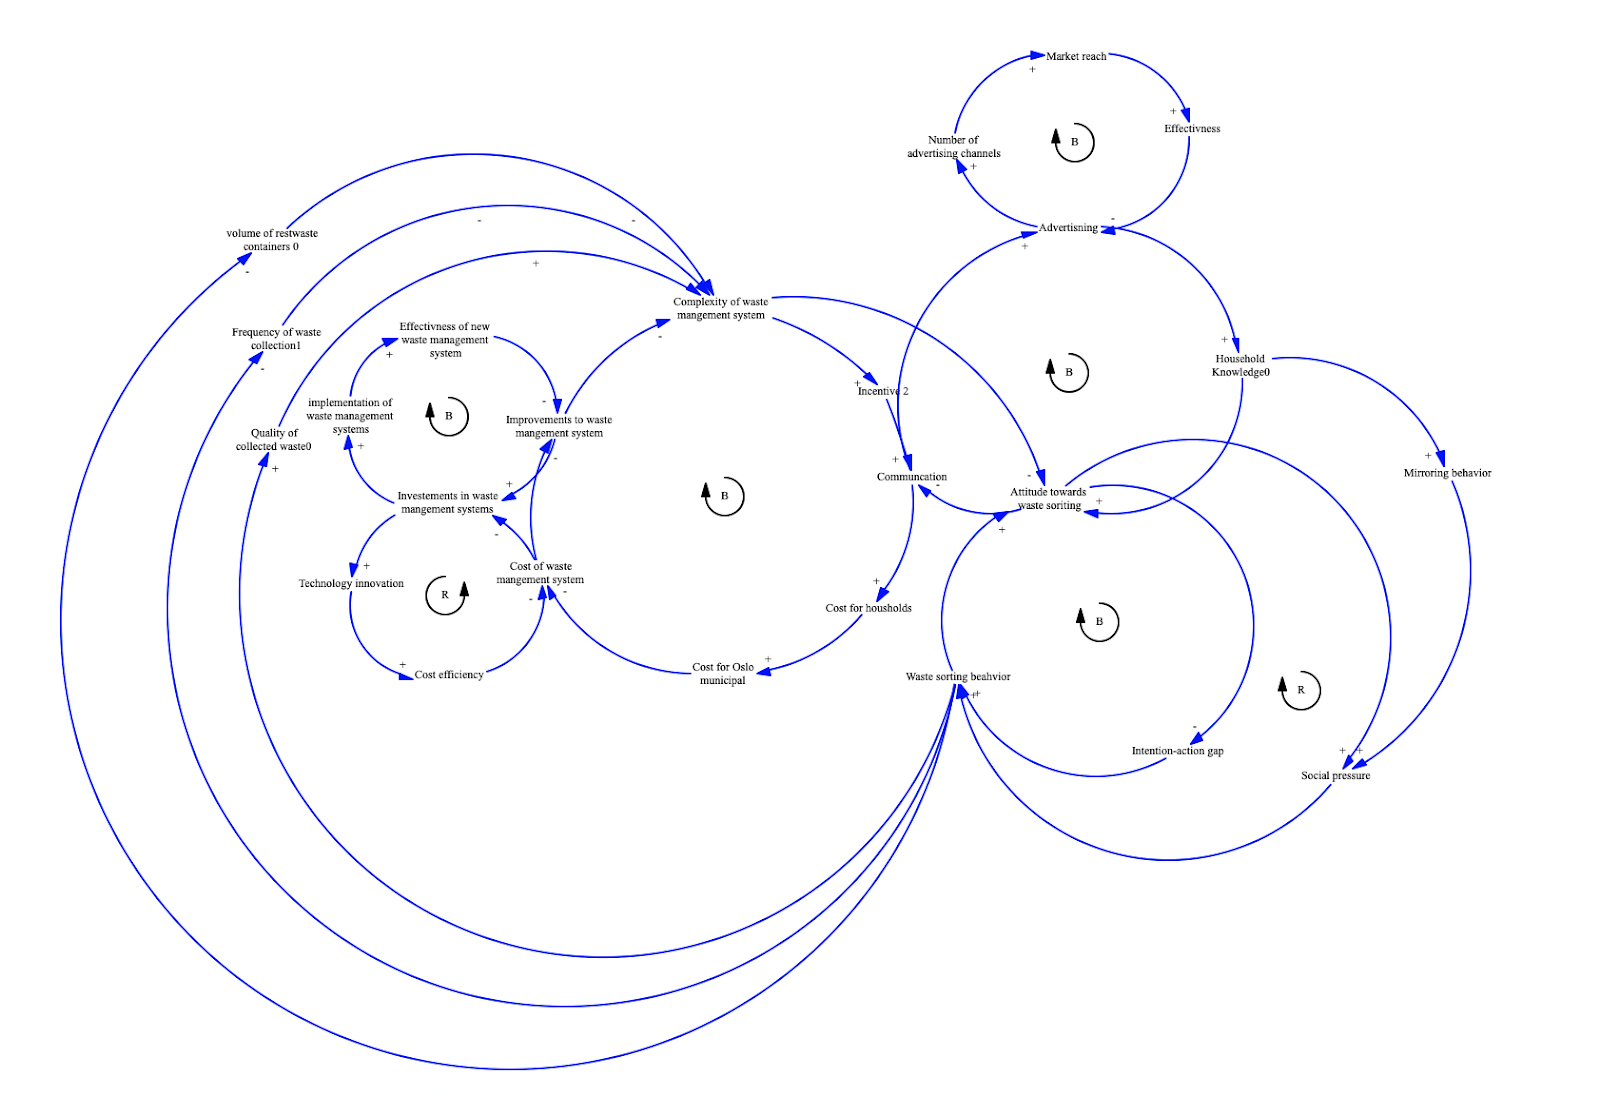
\includegraphics [scale=0.25,angle=90]{figures/fullcld.png}
\caption{Overview of The Causal Loop Diagram}
\label{fig:fullcld}
\end{figure}

\indent \newline
The three central variables in the causal loop diagram is "Quality of collected waste", "Frequency of waste collection" and "volume of rest waste containers". These variables represent initiatives which are among the most important factors in order to improve waste sorting behavior.  

\section{Complexity of Waste Management System}

\begin{figure}[H]
\centering
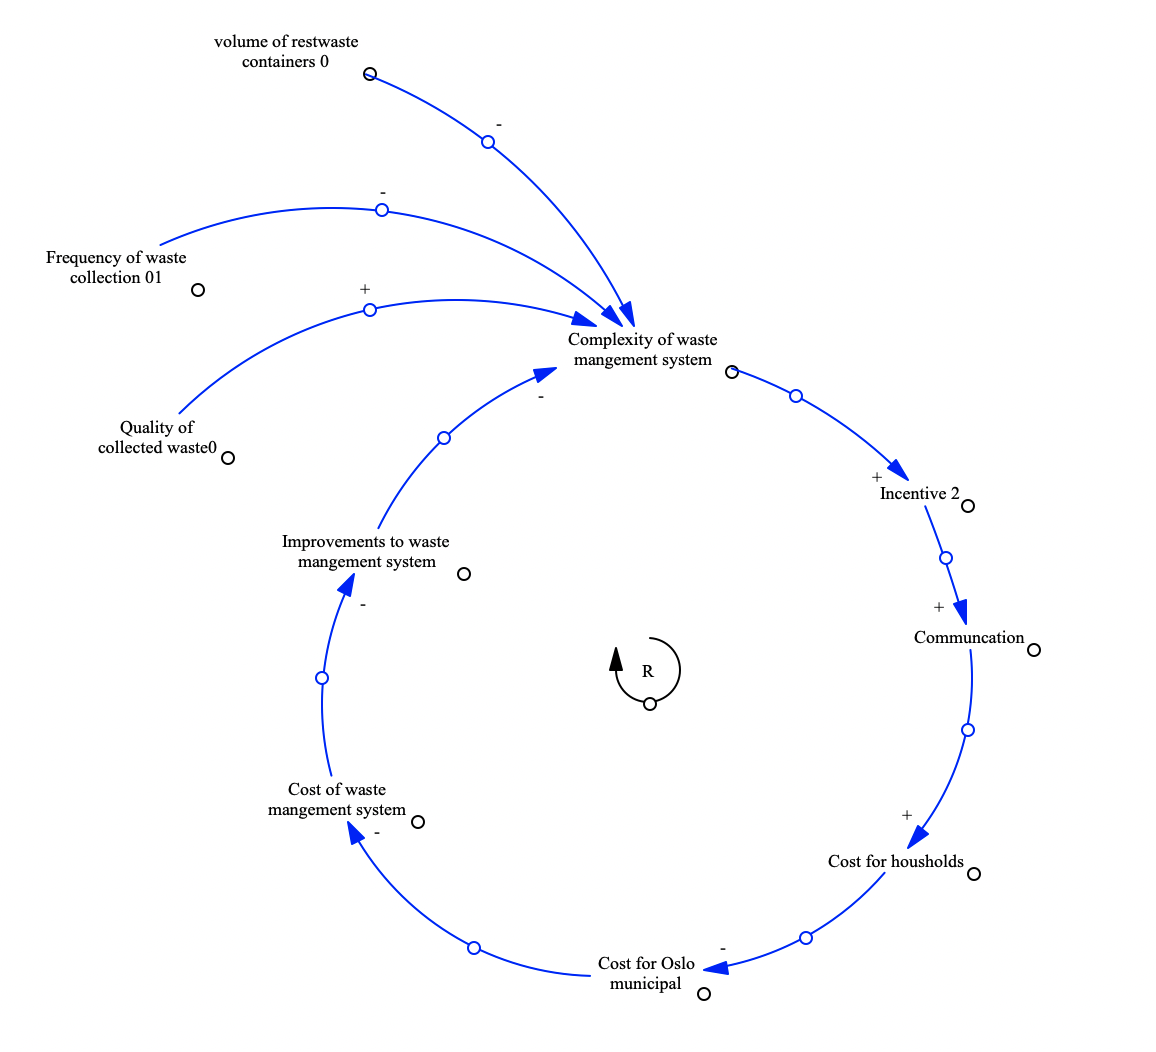
\includegraphics [scale=0.30,angle=360]{figures/complexity.png}
\caption{Complexity of The Waste Management System}
\label{fig:complexity}
\end{figure}

\indent \newline
The complexity of  the waste management system can be interpreted in two different ways.
One is assuming that the citizens have a waste container for each of the materials, which consists of paper, plastic, rest waste and food waste. In this case, Oslo municipality does not have to sort the waste and get rid of the intermediary where the waste is actually sorted. This means that the waste can be sent directly to recycling, which has a significant impact on the complexity of the system. From the citizens point of view, the complexity of the system will rise with the condition of high quality of collected waste. Increasing the frequency of waste collection leads to a less complex waste management system, whereas the citizens avoid bringing the waste back home, presuming the rest waste containers are fully loaded. This also applies to an increase in the volume of rest waste containers. An increase in the complexity of the system means that more incentives are needed on the basis that the citizens have to make more effort to sort properly. Therefore, more incentives mean more communication towards citizens. Possible incentives can presumptive be a fine or financial reward given the quality of the waste sorted.  

\indent \newline
If Oslo municipality increases communication to the citizens, the costs for household will also increase. It has to do with the fact that a percentage of communication costs are charged to households. In this case, the higher the costs for households, the lower the costs for Oslo municipal. The costs for the Oslo municipality are, among other variables, determined through economic incentives, communication and costs related to the waste management system.  

\indent \newline
Assuming an increase in total costs for Oslo municipally, the costs related to the waste management will decrease. This represents a situation where the municipality needs to spend their financial resources on other pressing issues. The next part of the loop shows that an increase in the costs of waste management system will decrease improvements to waste management system. This is a result of a smaller amount of the total budget going towards improvements. Once improvements to waste management systems increase, through technology innovation (explained in Figure 2.6), the complexity of waste management system will decrease. This leads to a reinforcing loop. 

\section{Attitude Towards Waste Sorting}

\begin{figure}[H]
\centering
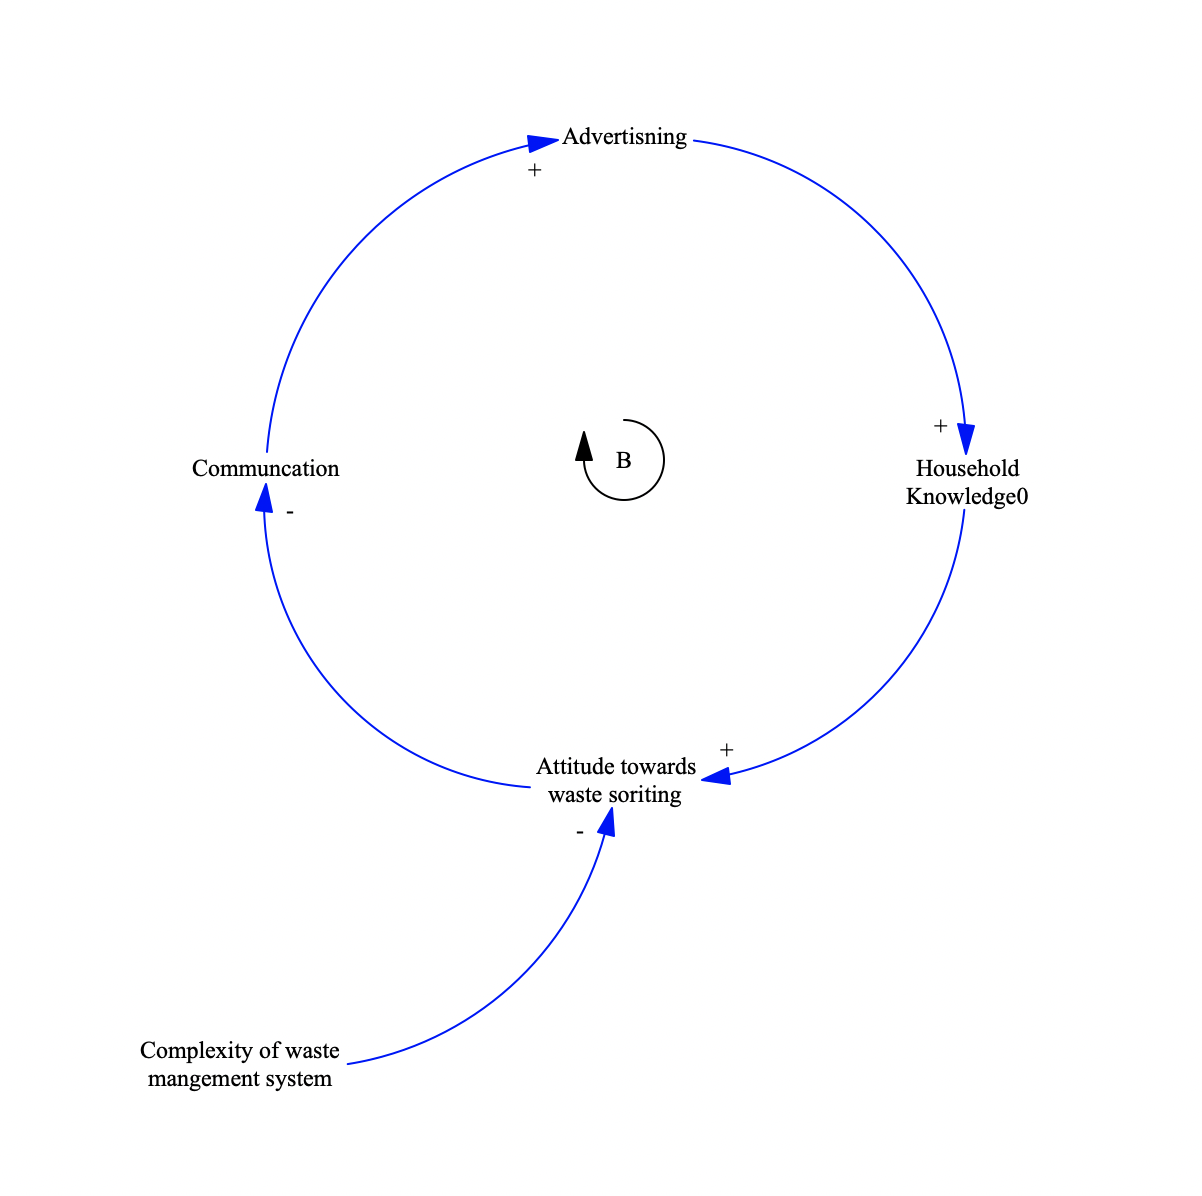
\includegraphics [scale=0.30,angle=360]{figures/attitude.png}
\caption{Attitude Towards Waste Sorting}
\label{fig:attitude}
\end{figure}

\indent \newline
Attitude towards waste sorting is an important variable in the causal loop diagram. The variable both affects and is affected by several variables, and is included in other sub-diagrams as well. Most of the effects related to complexity is explained above, but it also has an effect on the attitude towards waste sorting. If the waste management system increases in complexity, the target group's attitude towards waste sorting will most likely decrease. It is an essential factor for this target group that the waste management system is easy to understand and utilize, and that the workload for the household is minimized. 

\indent \newline
A crucial factor towards increasing the attitude towards waste sorting is household knowledge. When household knowledge is low, it is difficult to have a positive attitude towards waste sorting and vice versa. It is imperative for the target group to acquire knowledge on environmental-impact awareness, as well as the bin system, both curbside and in-house (what goes where). Therefore, it is necessary for the target group to have a reliable source of information in order to acquire a satisfying level of knowledge regarding waste sorting. This will have a positive effect on attitude towards waste sorting.

\indent \newline
There are currently several TV commercials and public posters related to material recycling. However, it is lacking advertising through additional media channels (Figure 2.4). The variables in figure 2.4 are connected through communication, which is a common denominator for the variables mentioned above. This is a simple, but effective balancing loop. If advertising is increased through various media channels, household knowledge will increase, which will lead to an increase in the attitude towards waste sorting. This connects back into communication and will reinforce the relationships even further.

\section{Advertising}

\begin{figure}[H]
\centering
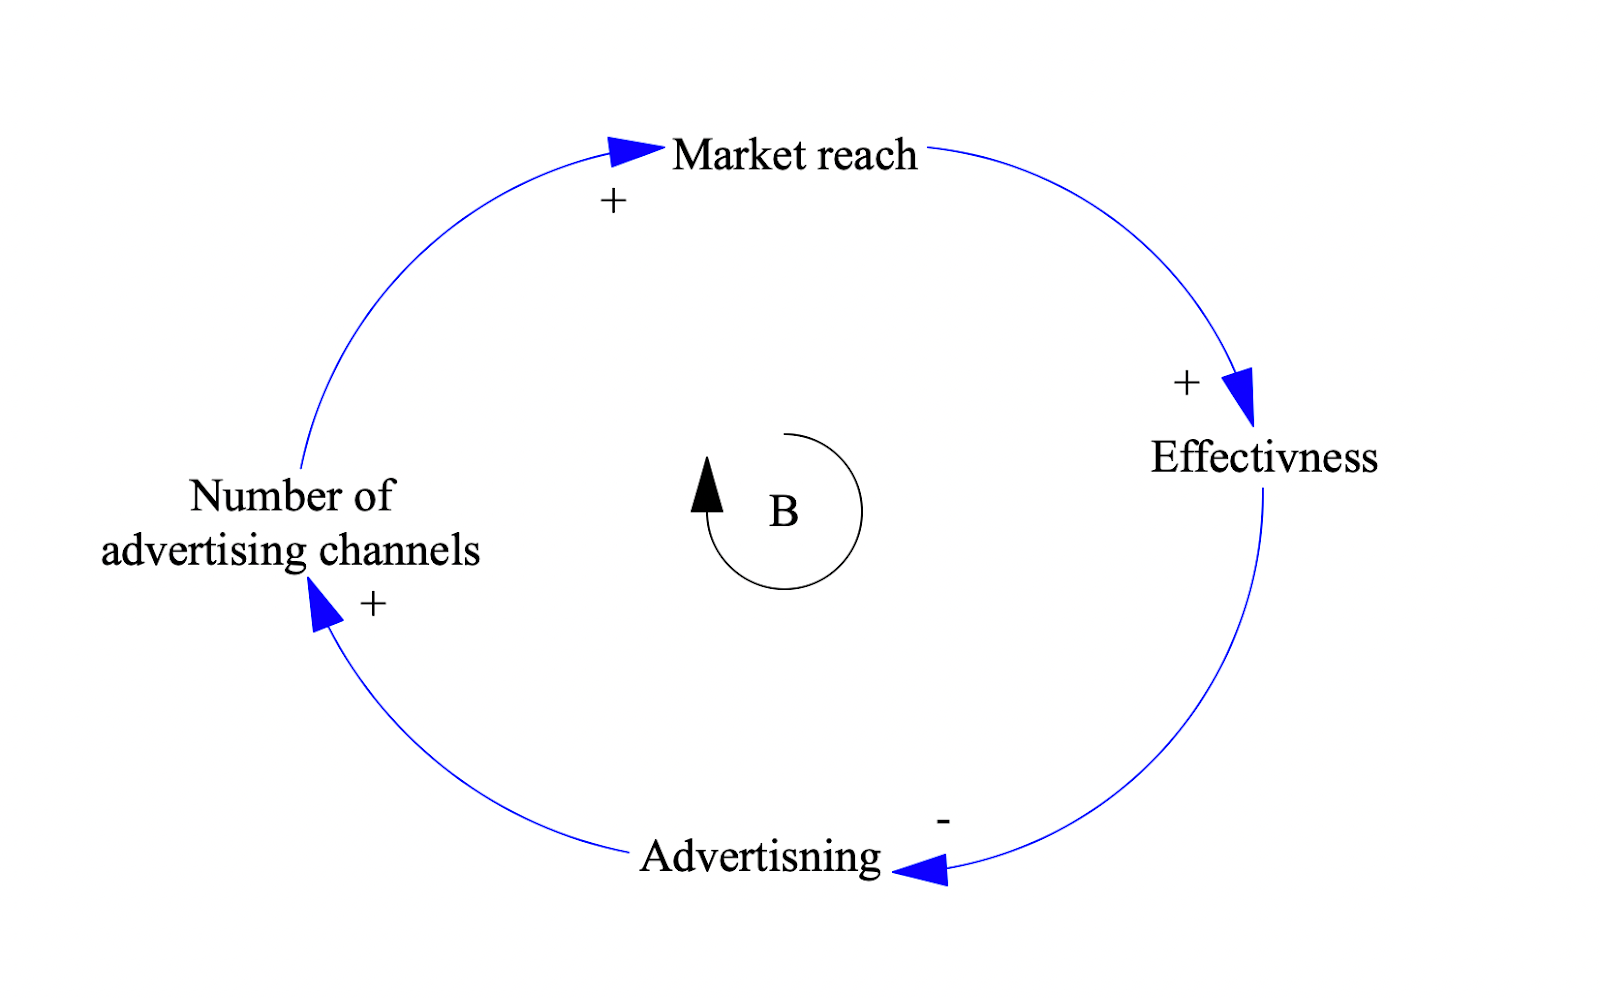
\includegraphics [scale=0.20,angle=360]{figures/advertising.png}
\caption{Advertising}
\label{fig:advertising}
\end{figure}

\indent \newline
In order to achieve the highest market reach within the intended target group, it is necessary to put emphasis on advertising. The target group lacks household knowledge, environmental-impact knowledge and awareness. A potential strategy, in order to reach out to the target group in the most effective way, is communication through various advertising channels. This means focusing on social media campaigns and more traditional advertising channels. Carefully selecting the ideal advertising channels is critical towards maximizing the market reach. Digital platforms such as Facebook, Snapchat, and Instagram is a good place to start. 

\indent \newline
The effect of increasing the number of advertising channels i.e Facebook, Snapchat, Instagram, Twitter, Tumblr, LinkedIn and YouTube, is an increase in market reach within the designated target group. The target group has a vast age interval, and the various social media platforms attract different age groups. Therefore, the more advertising channels, the higher market reach achieved. When the market reach is increased, the resulting outcome will be that the overall effectiveness of our advertising will increase. Once optimal effectiveness is reached, then less advertising is required in order to reach the same results. This part of the diagram results into a balancing loop. 

\section{Social Pressure \& The Intention-Action Gap}

\begin{figure}[H]
\centering
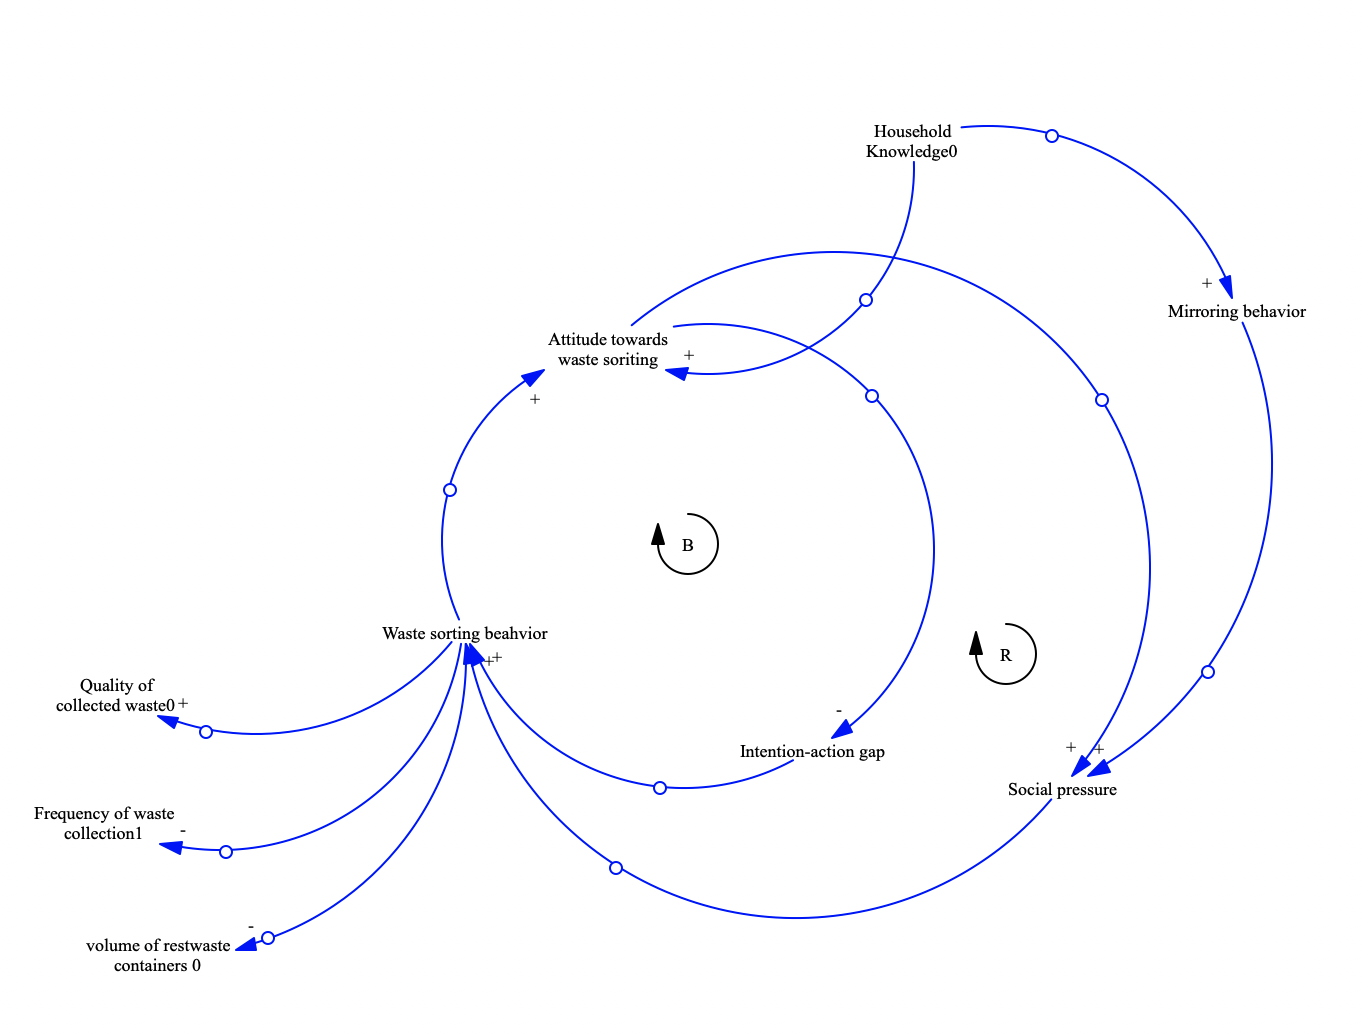
\includegraphics [scale=0.28,angle=360]{figures/socialpressure.png}
\caption{Social Pressure \& The Intention-Action Gap}
\label{fig:Social Pressure}
\end{figure}

\indent \newline
As mentioned formerly, attitude towards waste sorting and household knowledge is two imperative variables in the causal loop diagram, while improving waste sorting behavior is the main objective. However, these variables can lead to both positive and negative effects. 

\indent \newline
An increase in household knowledge will influence a portion of the members in the household to recycle correctly and develop enough awareness of the environmental impact. If one household member starts waste sorting correctly, one can presume that it leads to a mirroring behavior among the other members of the household. According to Jeff Thompson, mirroring behavior is something that occurs subconsciously, especially if we have a positive relationship with the subject \cite{mimicry}. This is often the case in households within this target group, living with either a spouse or friends. In addition, if household knowledge is increased, it will have a positive influence on the attitude towards waste sorting since the subject will be aware of the resulting effects of waste sorting.

\indent \newline
Mirroring behavior has a positive effect on social pressure. It is in our human nature to be sensitive to social pressure, and conform to the values, attitudes or behaviors of others. This can increase individual participation in recycling \cite{shackel}. Individuals will be influenced and encouraged by their fellow peers. This will directly affect their waste sorting behavior. Therefore, if social pressure increases, the waste sorting behavior will also increase.  

\indent \newline
Attitude towards waste sorting will also influence the intention-action gap. The intention-action gap represents the difference between what people say they do, and what they actually do \cite[p. 8]{intention}. Research shows that is common for the target group to have a large intention-action gap when it comes to waste sorting behavior. It amounts to motivation and commitment, which originates from the attitude towards waste sorting. In other words, if there is an increase in attitude towards waste sorting, it will decrease the intention-action gap because people are more committed to the cause. 

\indent \newline
Waste sorting behavior will influence the three variables; "quality of collected waste", "frequency of collected waste" and "volume of rest waste containers". There is a positive relationship between the quality of collected waste and waste sorting behavior. In the case where waste sorting behavior is improved, it will have a direct positive effect on the quality of collected waste. The target group will be more accurate and precise when it comes to waste sorting, which will result in better quality. Regarding the effect of waste sorting behavior on frequency of collected waste, it will have a negative connection. When waste sorting behavior is increased, it will result in less overflow of waste in the containers, which leads to a reduction in frequency of collected waste. It revolves around the household "optimizing" their waste in order to decrease the frequency of collected waste. 

\indent \newline
The relationship between waste sorting behavior and volume of rest waste containers represents the final part of the loop. When waste sorting behavior is increased, it will essentially make more space in the existing containers. The households will optimize their garbage bags, which will result in less excess garbage in various bags.  Therefore, there is a negative relationship between these two variables. 

\section{Improvements to Waste Management System}

\begin{figure}[H]
\centering
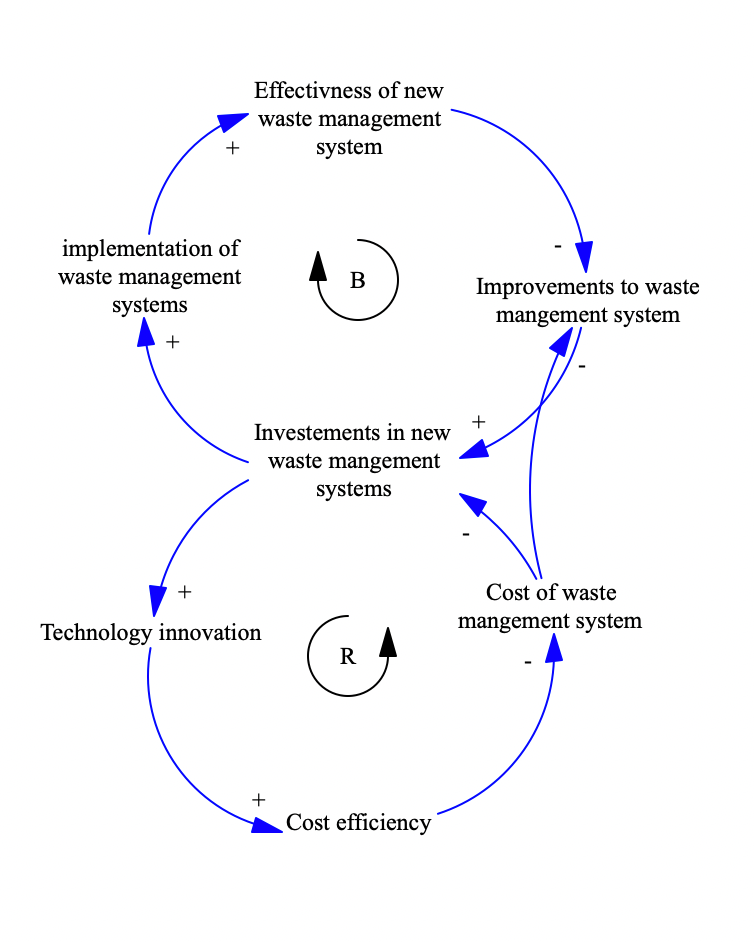
\includegraphics [scale=0.32,angle=360]{figures/improvements.png}
\caption{Improvements to Waste Management System}
\label{fig:improvements}
\end{figure}

\indent \newline
The final part of the causal loop diagram displays the relationships between variables related to how improvements can be made to the current waste management system. In order for this to happen, it is vital to raise enough capital. This can be obtained either from households, through economic incentives or funding from the government. If the effectiveness of the new waste management system increases, there is less need for making improvements to the system. With the condition of an improved sustainable waste management system, an increase in investments is necessary. If investments in the waste management system increases, then  opportunities related to technology innovations will follow. If there is more room to explore new innovations, the cost efficiency will rise, which will result in a decrease in the costs of the waste management system. This feeds back into both the investments in new waste management system and the improvements. The increase of investments leads to implementation of new waste management to establish a more sustainable system for recycling and waste collection. This feeds back into the effectiveness of new management systems, where effectiveness can be measured. The discussed variables and their relationships results into a balancing loop. 

\indent \newline
The causal loop diagram is a visual representation of interdependencies and feedback processes related to the waste management system. The following parts of the paper will convert the diagram into a stock and flow model to measure the resulting effects of proposed solutions, in order for Oslo municipality to reach their recycling goals.


\chapter{Equation Analysis}
To provide a better understanding of the stock and flow model, the following section will explain the equations of some of the most important variables, which influence waste sorting behavior and ultimately the material recycling percentage. 

\section{Change in Frequency \& Frequency of Waste Collection}

\begin{figure}[H]
\centering
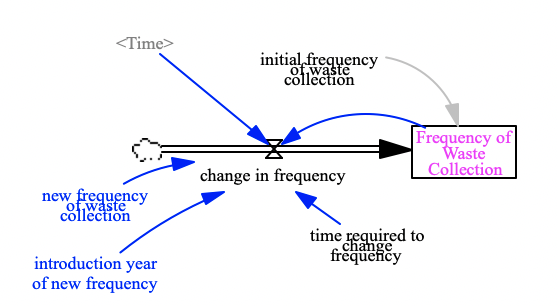
\includegraphics [scale=0.34,angle=360]{figures/frequency.png}
\caption{Change in Frequency \& Frequency of Waste Collection}
\label{fig:frequency}
\end{figure}	

\indent \newline
Change in frequency is modeled as an inflow and measures change in frequency over a period of time. The equation in the inflow "change in frequency" states that if time is less than the introduction of new frequency, then the value of change in frequency will be 0. If the introduction year of new frequency is greater than or equal to time, then the model computes the change in frequency per year (new frequency of waste collection- frequency of waste collection)/time required to change frequency. The frequency of waste collection is formulated as a stock and represents the frequency of waste collection at a specific time. 

\section{Complexity of Waste Management System}

\begin{figure}[H]
\centering
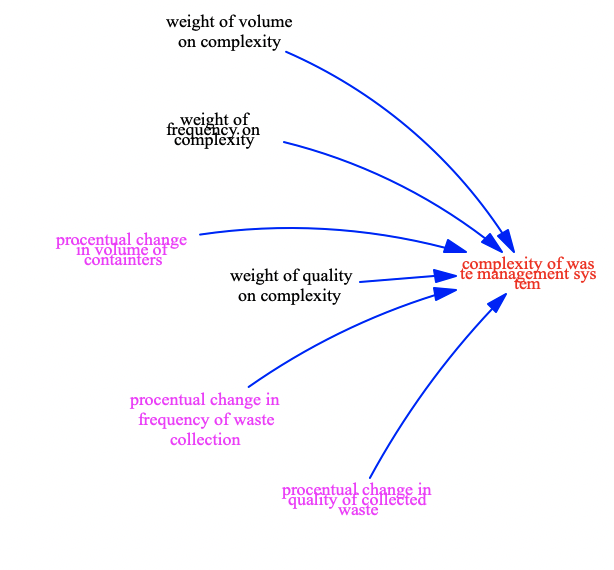
\includegraphics [scale=0.34,angle=360]{figures/complexityeq.png}
\caption{Complexity of Waste Management System}
\label{fig:complexityeq}
\end{figure}

\indent \newline
The variable "Complexity of waste management system" is a weighted average of three exogenous "weight" variables and their related three endogenous variables. The exogenous variables are weighted differently, which is based on the variable's impact on complexity of waste management system. If there is an increase in volume or frequency, the complexity decreases. This is due to  waste containers not overflowing with waste. When quality increases, the complexity increases since there are additional containers that complicate waste sorting. 

\section{Waste Sorting Behavior}

\subsection{Potential Waste Sorting Behavior}

\begin{figure}[H]
\centering
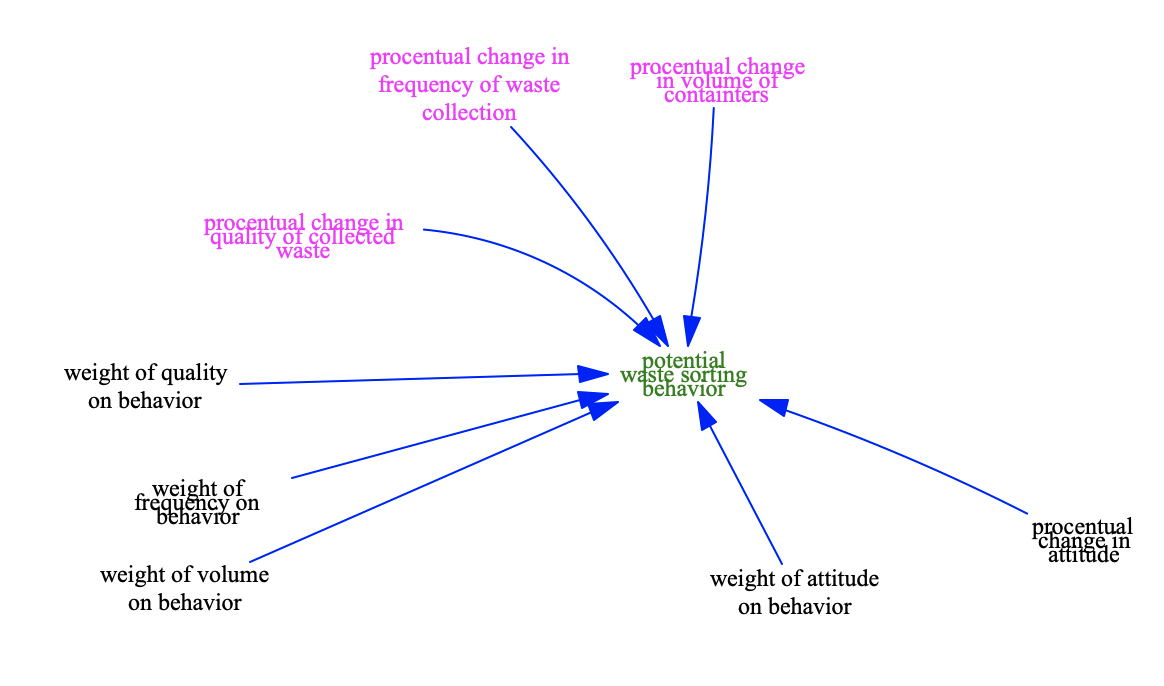
\includegraphics [scale=0.26,angle=360]{figures/potentialbehaviour.png}
\caption{Potential Waste Sorting Behaviour}
\label{fig:potentialbehaviour}
\end{figure}

\indent \newline
The endogenous variable "potential waste sorting behavior" computes the level of the potential sorting behavior. The equation shows that an increase in the volume of the rest waste containers decreases potential waste sorting behavior. A larger volume makes it easier for the citizens to throw everything in one container. An increase in quality and attitude  have a positive effect on potential waste sorting behavior. Additionally the equation states that an increase in the frequency of waste collection will have a positive effect on potential waste sorting behavior. The reason for this is that an increase in frequency will make it less likely that the waste containers will overflow. On the other hand, if the rest waste containers are full, the citizens will most likely throw the waste in the wrong container or just leave the waste next to the containers. 

\subsection{Change in Waste Sorting Behaviour}

\begin{figure}[H]
\centering
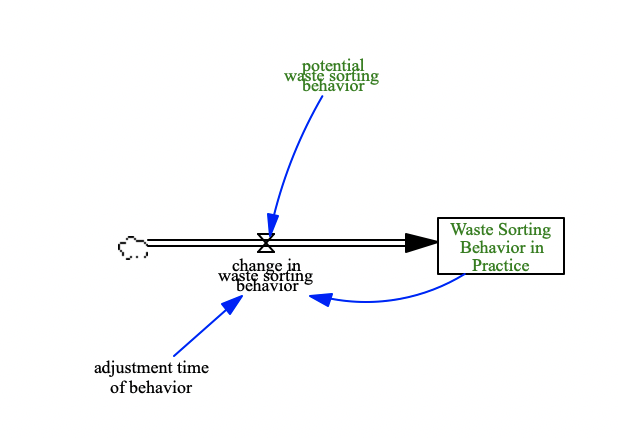
\includegraphics [scale=0.34,angle=360]{figures/changebehaviour.png}
\caption{Change in Waste Sorting Behavior \& Waste Sorting Behavior in Practice}
\label{fig:changebehaviour}
\end{figure}

\indent \newline
The variable "change in waste sorting behavior" is modeled as an inflow to measure the change of waste sorting behavior over a period of time. The equation defines the change in waste sorting behavior per year. 

\subsection{Waste Sorting Behavior in Practice}

\indent \newline
Waste sorting behavior is represented as a stock in the existing model. The stock measures the level of waste sorting behavior at a specific time, and is influenced by the change in waste sorting behavior.

\section{Plastic in Households}

\subsection{Inflow Plastic in Households}

\begin{figure}[H]
\centering
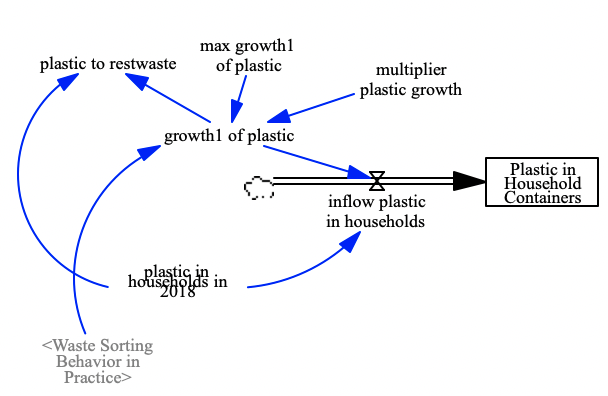
\includegraphics [scale=0.34,angle=360]{figures/plasticinflow.png}
\caption{Plastic in Households}
\label{fig:plasticinflow}
\end{figure}

\indent \newline
The variable "inflow plastic in households" is an inflow because it measures the rate of change in plastic in household containers. The equation computes the tons of plastic per year the household throws in the garbage and is affected by "growth1" in plastic and "plastic in household 2018".

\subsection{Growth1 of Plastic}

\indent \newline
The endogenous variable  "growth1 of plastic" is modeled as a minimum function that estimates the smallest values between the exogenous variable "max growth1 of plastic" and the stock "waste sorting behavior in practice", multiplied with the exogenous variable "multiplier plastic growth". The function gives an indication of how great the citizens are at sorting plastic. The minimum function also prevents the function from going negative. 

\subsection{Plastic to Rest Waste}

\indent \newline
The endogenous variable "plastic to rest waste" indicates the amount of plastic that is going into the rest waste. The equation takes the amount of plastic in households 2018 and multiplies it with 1 - growth1 of plastic. "Growth1 of plastic" suggests to what extent the citizens are sorting plastic. An increase in the value of the growth1 variable indicates that they are improving at sorting plastic. 

\subsection{Growth2 of Plastic}

\begin{figure}[H]
\centering
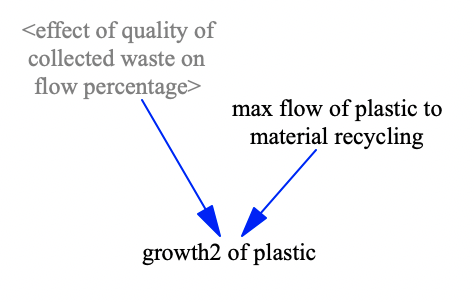
\includegraphics [scale=0.34,angle=360]{figures/plasticgrowth.png}
\caption{Growth2 of Plastic}
\label{fig:plasticgrowth}
\end{figure}

\indent \newline
"Growth2 of plastic" is formulated as an endogenous variable. The variable's equation is a minimum function, which calculates the smallest value of "max flow of plastic to material recycling" or "0.59 * effect of quality of collected waste on flow percentage". The minimum function also helps prevent the function from going negative.





\chapter{Development of Simulation Model}
\section{Stocks}

\indent \newline
The existing simulation model is expanded through adding new stocks and flows, as well as the relations from the causal loop diagram. The expanded model consists of the most important variables, when it comes to improving waste sorting behavior and the material recycling rate. The added stocks results in a better understanding of how these variables can be influenced. Some of the variables from the causal loop diagram were changed into stocks based on these criteria:

\indent \newline
\begin{enumerate}
\item The units of measure are usually a quantity, and difficult to change in a moment.
\item Should give the system inertia.
\item	If the variable represents a behavior which is important in the dynamics we want to explain. 
\cite[p. 192]{system}
\end{enumerate}


\indent \newline
The following variables were converted directly into stocks; household knowledge, advertising and improvements to waste management system. These are in turn influenced by other variables and causal links from the causal loop model. Primarily, the variable household knowledge was added directly into the model as a stock. Studies show that household knowledge leads to a better attitude towards waste sorting, which will have a positive effect on waste sorting behavior \cite[p. 13, Preliminary report]{intention}.The variable "improvements to waste management system" from the causal loop diagram was converted into the stock "waste management system in practice". The stock represents improvements and changes made to the waste management system. The model accumulates the change in the system over time. Lastly, the stock "advertising effectiveness in practice" was added in order to measure the effect on attitude. 

\section{Values}

\indent \newline
The original waste supply chain model was designed for simulating the material recycling rate for the total population. Since this paper focuses on 20-39 year old's, not coming from Asia, Africa, Latin-America and Eastern Europe outside of EU, it has been necessary to make some adjustments. For the model to represent the intended target group, values have been changed in some of the variable’s associated equations.

\indent \newline
The following variables have been tweaked: "paper in households 2018", "food in households 2018", "plastic in households 2018", "rest waste in households 2018", "other energy inflows" and "other material inflows". All of the mentioned variable's initial values have been multiplied with 0.27, because the target group represents 27\% of Oslo's population. 

\section{Main Systems}

\indent \newline
By adding the variables from the causal loop diagram, the stock and
flow model increases in complexity. Because of this, the model is split 
into eight main systems: 

\indent \newline
\begin{enumerate}
\item Improvements in waste management system
\item Complexity
\item Costs 
\item Communication and advertising 
\item Household knowledge
\item Social pressure/behaviour
\item Attitude towards waste sorting
\item Waste sorting behaviour
\end{enumerate} 

\indent \newline
The improvements in waste management system (1) demonstrates how investments and technology innovation can improve the waste management system in practice. Two resulting initiatives from investments and innovations are a new volume of containers and a new frequency of waste collection. There is also an exogenous initiative, which consists of improving the quality of collected waste. The system displays the procentual change in the stocks and how they affect the complexity and costs of the waste management system, as well as the potential waste sorting behavior. 

\indent \newline
The second part of the model describes the complexity (2) of the waste management system and its direct and indirect effect on the potential attitude towards sorting waste. The model calculates the complexity of the waste management system through a weighted average of the three initiatives described above and improvements in waste management system in practice.

\indent \newline
The next part of the model explains how the different initiatives and improvements/factors contribute to the costs of the waste management system (3). The subsystem shows how the costs are divided between Oslo municipality and the households, and measures the effect household costs has on the potential attitude towards sorting waste.

\indent \newline
Communication and advertising (4) are two other factors in the model which have a potential effect on attitude towards sorting waste. Communication is dependent on the complexity of the waste management system, and influence both costs and potential attitude towards waste sorting. Through the number of advertising channels and market reach, the model calculates the effect of advertising on household knowledge and the potential attitude towards sorting waste. 

\indent \newline
Household knowledge (5) is influenced by advertising and affects mirroring behavior and the potential attitude towards sorting waste. Social pressure (6) is influenced by mirroring behavior and the attitude towards sorting waste in practice. It affects the potential waste sorting behavior. 

\indent \newline
A summarizing part of the model is the attitude towards sorting waste system (7) and waste sorting behavior (8). This section shows how all of the effects in the model changes the attitude towards sorting waste in practice, which includes effects from complexity, incentives, costs, communication, advertising and household knowledge. This leads to the purpose of the simulation model, which is to improve waste sorting behavior in practice. The stock represents the influence from attitude towards sorting waste in practice, the intention-action gap variable and the initiatives from the first section of the model.

\indent \newline
The following part of the chapter displays the main systems, where new variables and stocks have been added, and where changes have been made to values and equations. The section explains the different equations in detail and the reasoning behind certain values. Variables which hold values equal to one are not commented on, since their only purpose is holding a variable's starting value.

\section{Formulations and Comments}
\subsection{Improvements in Waste Management System}
\begin{figure}[H]
\centering
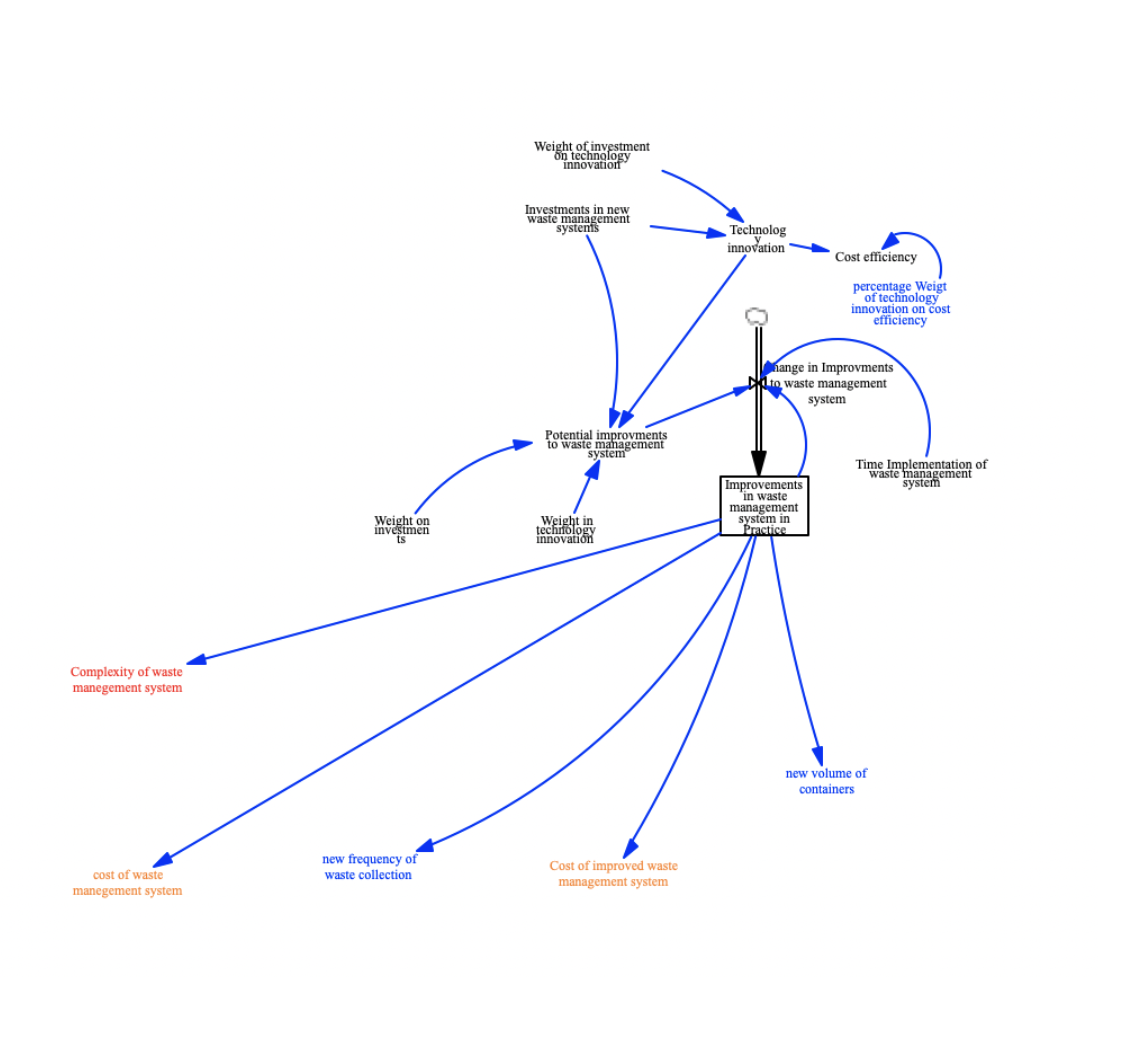
\includegraphics [scale=0.38,angle=360]{figures/improvementsystem.png}
\caption{Improvements System}
\label{fig:improvementsystem}
\end{figure}

\begin{flalign}
&\textbf{Technology innovation} =  &&  \text{[Dimensionless]}\nonumber\\
&I \times W && \nonumber
\end{flalign} 
\textit{Where:
\begin{itemize}
    \item[] $I$ =  Investments in new waste management systems
    \item[] $W$ = Weight of investments on technology innovation
\end{itemize}
}
\indent \newline
The endogenous variable technology innovation is dependent on the number of investments multiplied with how much of the new investments that leads to technological innovations. 

\begin{flalign}
&\textbf{Cost efficiency} =  &&  \text{[Dimensionless]}\nonumber\\
&TI \times W && \nonumber
\end{flalign} 
\textit{Where:
\begin{itemize}
    \item[] $TI$ = Technology innovation
    \item[] $W$ = Percentage weight of technology innovation on cost efficiency
\end{itemize}
}
\indent \newline
Cost efficiency is dependent on the weight of technology innovation which reduces the waste management system costs.

\begin{flalign}
&\scriptstyle\textbf{Percentage weight of technology innovation on cost efficiency} = 0.2 && \nonumber \text{[Dimensionless]}
\end{flalign} 
\indent \newline
The model assumes that 20 percent of technology innovation relates to improving cost efficiency. 

\begin{flalign}
&\textbf{Costs of waste management system} = && \text{[Dimensionless]}\nonumber\\
&1 + \frac{- PV \times WV + PF \times WF + PQ \times WQ - CE \times WC} {WV + WF + WQ - WC} && \nonumber
\end{flalign}
\textit{Where:
\begin{itemize}
    \item[] $PV$ = Procentual change in volume of containers
    \item[] $WV$ = Weight of volume on costs
    \item[] $PF$ = Procentual change in frequency of waste collection
	\item[] $WF$ = Weight of frequency on costs
	\item[] $PQ$ = Procentual change in quality of collected waste
	\item[] $WQ$ = Weight of quality on costs
	\item[] $CE$ = Cost efficiency
	\item[] $WC$ = Weight of cost efficiency
\end{itemize}
}
\indent \newline
Costs of the waste management system estimates a weighted average of the procentual change in volume of containers, frequency of waste collection, quality of collected waste and cost efficiency. The procentual change in volume of containers and cost efficiency reduce the costs, while the two other initiatives increase the costs. 

\begin{flalign}
&\textbf{Potential improvements to waste management system}= && \text{[Dimensionless]}\nonumber\\
&1 + \frac{I \times WI + TI \times WT} {WI +WT} && \nonumber
\end{flalign} 
\textit{Where:
\begin{itemize}
    \item[] $I$ = Investments in new waste management system
    \item[] $WI$ = Weight on investments
    \item[] $TI$ = Technology innovation
	\item[] $WT$ = Weight on technology innovation
\end{itemize}
}
\indent \newline
The model assumes that the potential improvements to the waste management system is dependent on a weighted average of investments and technology innovation.

\begin{flalign}
&\scriptstyle\textbf{Change in improvements to waste management system}= && \text{[Dimensionless/Year]}\nonumber\\
&\scriptstyle\frac{PI - I} {TI} && \nonumber
\end{flalign} 
\textit{Where:
\begin{itemize}
    \item[] $PI$ = Potential improvements to waste management system
    \item[] $I$ = Improvements in waste management system in practice
    \item[] $TI$ = Time implementation of waste management system
\end{itemize}
}
\indent \newline
The change in improvements to the waste management system is an inflow that estimates the change in improvements in the waste management system per year. 

\begin{flalign}
&\scriptstyle\textbf{Improvements in waste management system in practice}=&& \text{[Dimensionless]}\nonumber\\
&\scriptstyle\int_{0}^{t} \text{Change in improvements to waste management system} \times dt && \nonumber
\end{flalign}
\indent \newline
Improvements in waste management system in practice calculates the level of the improvements. The stock is influenced by the inflow change in improvements to waste management system.

\begin{flalign}
&\textbf{Costs of improved waste management system}=&& \text{[Dimensionless]}\nonumber\\
&\text{Improvements in waste management system in practice} && \nonumber
\end{flalign}
\indent \newline
Costs of improved waste management system is dependent on improvements in waste management system in practice. The variable represents the added costs from the improvements. 

\begin{flalign}
&\textbf{Complexity of waste management system}=&& \text{[Dimensionless]}\nonumber\\
&1 + \frac{- PV \times WV - PF \times WF + PQ \times WQ - (WI \times I - 1)} {WV + WF + WQ + WI} && \nonumber
\end{flalign} 
\textit{Where:
\begin{itemize}
    \item[] $PV$ = Procentual change in volume of containers
    \item[] $WV$ = Weight of volume on complexity
    \item[] $PF$ = Procentual change in frequency of waste collection
	\item[] $WF$ = Weight of frequency on complexity
	\item[] $PQ$ = Procentual change in quality of collected waste
	\item[] $WQ$ = Weight of quality on complexity
	\item[] $I$ = Improvements in waste management system in practice
	\item[] $WI$ = Weight of improvements in waste management system on complexity
\end{itemize}
}
\indent \newline
The complexity of waste management system is dependent on a weighted average of the procentual change in volume of containers, frequency of waste collection, quality of collected waste and improvements in waste management system in practice. The procentual change in volume of containers, frequency of waste collection and improvements in waste management system in practice reduces complexity, while the procentual change in quality of collected waste increases the complexity.

\begin{flalign}
&\textbf{New volume of containers}= && \text{[Dimensionless]}\nonumber\\
&\text{IF THEN ELSE}(I > 2, 1 - (PV \times I - 1), 1) && \nonumber
\end{flalign} 
\textit{Where:
\begin{itemize}
    \item[] $I$ = Improvements in waste management system in practice
    \item[] $PV$ = Percentage change in volume from new investment
\end{itemize}
}
\indent \newline
The new volume of containers is an IF THEN ELSE function, which is calculated in the following way; if improvements in waste management system in practice is larger than two, we estimate the procentual change in volume in containers from new investment. If improvements in waste management systems in practice is smaller or equal to two, the new volume of containers is unchanged. 

\begin{flalign}
&\textbf{New frequency of waste collection}= && \text{[Dimensionless]}\nonumber\\
&\text{IF THEN ELSE}(I > 2, 1 - ((I - 1) \times WI), 1) && \nonumber
\end{flalign} 
\textit{Where:
\begin{itemize}
    \item[] $I$ = Improvements in waste management system in practice
    \item[] $WI$ = Weight of improvements on frequency
\end{itemize}
}
\indent \newline
The new frequency of waste collection is calculated through an IF THEN ELSE function. If improvements in waste management system in practice is greater than two, the model computes improvements in waste management system in practice - 1, which is multiplied with the weight of improvements on frequency. If waste management system in practice is less than or equal to two, the new frequency of waste collection is unchanged.  

\subsection{Advertising System}

\begin{figure}[H]
\centering
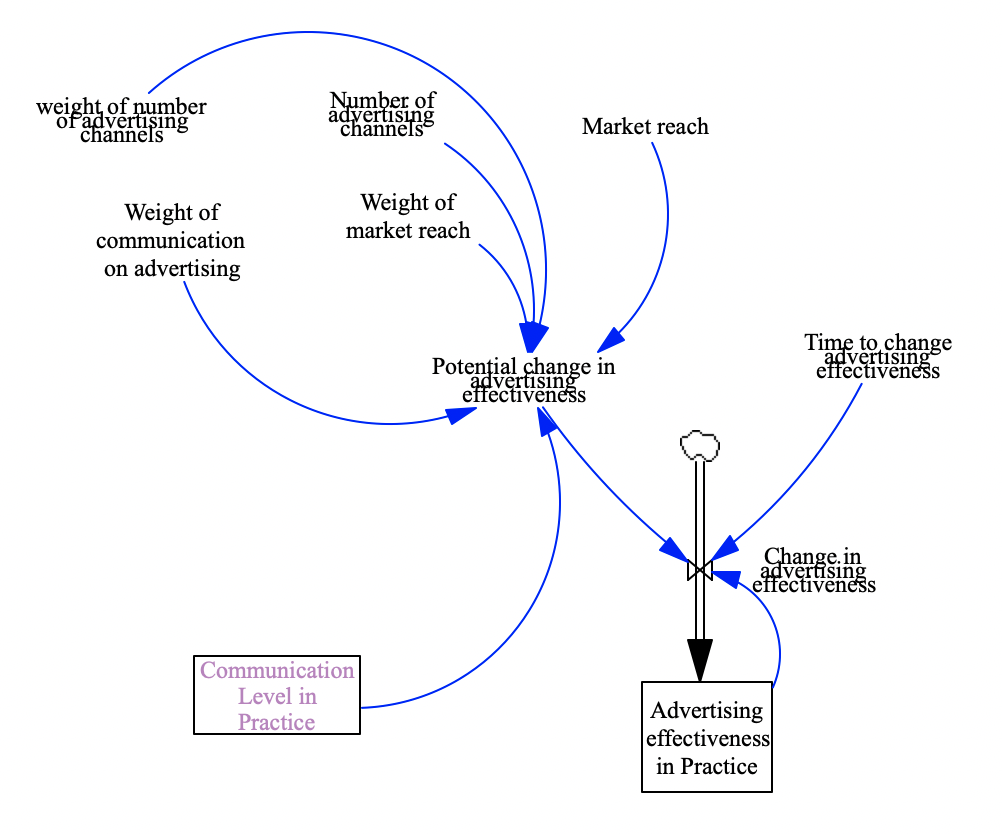
\includegraphics [scale=0.28,angle=360]{figures/advertisingsystem.png}
\caption{Advertising System}
\label{fig:advertisingsystem}
\end{figure}

\begin{flalign}
&\textbf{Communication level in practice}=&& \text{[Dimensionless]}\nonumber\\
&\int_{0}^{t}\text{Change of communication to citizens} \times dt && \nonumber
\end{flalign}
\indent \newline
The model assumes that the communication level in practice comes from changes in communication to citizens.

\begin{flalign}
&\textbf{Potential change in advertising effectiveness}=&& \text{[Dimensionless]}\nonumber\\
&1 + \frac{ C \times WC - 1 + A \times WA + M \times WM}  {WC + WA + WM} && \nonumber
\end{flalign} 
\textit{Where:
\begin{itemize}
    \item[] $C$ = Communication level in practice
    \item[] $WC$ = Weight of communication on advertising
    \item[] $A$ = Number of advertising channels
	\item[] $WA$ = Weight of number of advertising channels
	\item[] $M$ = Market reach
	\item[] $WM$ = Weight of market reach
\end{itemize}
}
\indent \newline
The potential change in advertising effectiveness is a weighted average of communication level in practice, the number of advertising channels, advertisements market reach and how they are weighted. This computes the level of advertising effectiveness per year.

\begin{flalign}
&\textbf{Time to change advertising effectiveness}= 4 && \text{[Year]}\nonumber\\
\nonumber
\end{flalign}
\indent \newline
The model assumes that the average time for advertising to be effective is four years.

\begin{flalign}
&\textbf{Change in advertising effectiveness}= && \text{[Dimensionless/Year]}\nonumber\\
&\frac{PA - A} {TA} && \nonumber
\end{flalign} 
\textit{Where:
\begin{itemize}
    \item[] $PA$ = Potential change in advertising effectiveness
    \item[] $A$ = Advertising effectiveness in practice
    \item[] $TA$ = Time to change advertising effectiveness
\end{itemize}
}
\indent \newline
The change in advertising effectiveness determines how effective the advertising has been per year. 

\begin{flalign}
&\textbf{Advertising effectiveness in practice}= && \text{[Dimensionless]}\nonumber\\
&\int_{0}^{t} \text{Change in advertising effectiveness} \times dt && \nonumber
\end{flalign}
\indent \newline
Advertising effectiveness in practice reports how effective the advertising campaign has been. The stock is influenced by the inflow change in advertising effectiveness. 

\subsection{Knowledge, Social Pressure, Attitude \& Behavior System}

\begin{figure}[H]
\centering
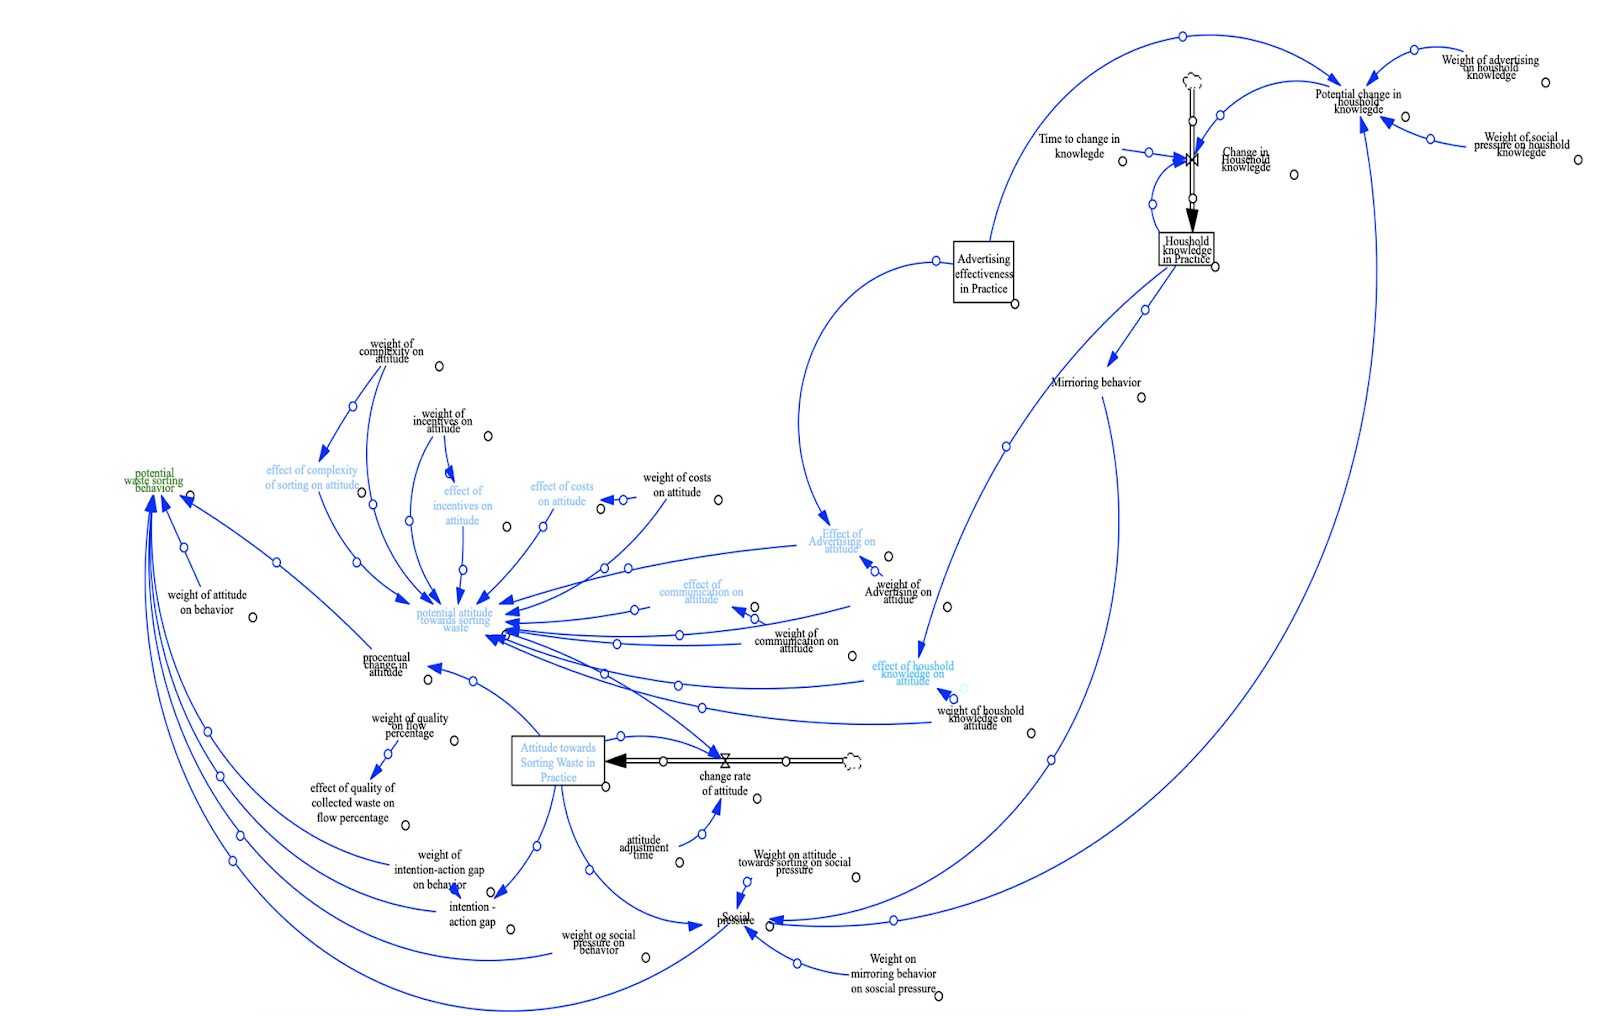
\includegraphics [scale=0.22,angle=360]{figures/lastsystem.png}
\caption{Knowledge, Social Pressure, Attitude \& Behavior}
\label{fig:lastsystem}
\end{figure}

\begin{flalign}
&\textbf{Potential change in household knowledge}= && \text{[Dimensionless]}\nonumber\\
&1 + \frac{ A \times WA - 1 + S \times WS}  {WA + WS} && \nonumber
\end{flalign} 
\textit{Where:
\begin{itemize}
    \item[] $A$ = Advertising effectiveness in Practice
    \item[] $WA$ =Weight of advertising on household knowledge
    \item[] $S$ = Social pressure
	\item[] $WS$ = Weight of social pressure on household knowledge
\end{itemize}
}
\indent \newline
The potential change in household knowledge is a weighted average of advertising effectiveness in practice, social pressures and how they are weighted. This shows how much advertising and social pressure change the knowledge of the households.  

\begin{flalign}
&\textbf{Time to change household knowledge} = 4 && \nonumber \text{[Year]}
\end{flalign} 
\indent \newline
The model assumes that it takes four years to achieve a change in household knowledge.

\begin{flalign}
&\textbf{Change in household knowledge}= && \text{[Dimensionless/Year]}\nonumber\\
&\frac{PH - H} {TH} && \nonumber
\end{flalign} 
\textit{Where:
\begin{itemize}
    \item[] $PH$ = Potential change in household knowledge
    \item[] $H$ = Household knowledge in practice
    \item[] $TH$ = Time to change household knowledge
\end{itemize}
}
\indent \newline
The change in household knowledge determines how effective advertising and social pressure has been on household knowledge per year.

\begin{flalign}
&\textbf{Household knowledge in practice}=&& \text{[Dimensionless]}\nonumber\\
&\int_{0}^{t}\text{Change in household knowledge} \times dt && \nonumber
\end{flalign}
\indent \newline
Household knowledge in practice reports the amount of knowledge the households have each year. The stock is influenced by the inflow change in household knowledge. 

\begin{flalign}
&\textbf{Weight of attitude towards sorting on social pressure} = 2 && \nonumber \text{[Dimensionless]}
\end{flalign} 
\indent \newline
The weight of attitude towards sorting on social pressure demonstrates the effect of attitude on social pressure. We conclude that attitude has a great influence on social pressure.

\begin{flalign}
&\textbf{Weight of advertising on household knowledge} = 3 && \nonumber \text{[Dimensionless]}
\end{flalign} 
\indent \newline
The weight of advertising on household knowledge determines how effective advertising is on household knowledge. We assume that advertising has a considerably larger impact on household knowledge than social pressure, since the target group utilizes substantial time on social media. 

\begin{flalign}
&\scriptstyle\textbf{Percentage of household knowledge who mirror behavior} = 0.1 && \nonumber \text{[Dimensionless]}
\end{flalign} 
\indent \newline
We assume that 10 percent of the target group mirrors others behavior towards waste sorting.

\begin{flalign}
&\textbf{Mirroring behaviour} = && \text{[Dimensionless]} \nonumber\\
&(H - 1) \times WH && \nonumber
\end{flalign} 
\textit{Where:
\begin{itemize}
    \item[] $H$ = Household knowledge in practice
    \item[] $WH$ = Weight of household knowledge on mirroring behavior
\end{itemize}
}
\indent \newline
Mirroring behavior is defined by household knowledge in practice multiplied with the weight of household knowledge. The function estimates how many with knowledge about waste sorting who can use mirroring to impact others.

\begin{flalign}
&\textbf{Social pressure}= && \text{[Dimensionless]} \nonumber\\
&1 + \frac{ A \times WA - 1 + M \times WM}  {WA + WM} && \nonumber 
\end{flalign} 
\textit{Where:
\begin{itemize}
    \item[] $A$ = Attitude towards sorting waste in practice
    \item[] $WA$ =Weight of attitude towards sorting on social pressure
    \item[] $M$ = Mirroring behavior
	\item[] $WM$ = Weight of mirroring behavior on social pressure
\end{itemize}
}
\indent \newline
Social pressure is a weighted average of attitude towards sorting waste in practice, mirroring behavior and how they are weighted. This computes the level of social pressure towards waste sorting. 

\begin{flalign}
&\textbf{Weight of advertising on attitude} = 3 && \nonumber \text{[Dimensionless]}
\end{flalign} 
\indent \newline
The weight of advertising on attitude determines how effective advertising is on attitude. We believe that advertising has a crucial effect on attitude due to our target group spending substantial time on social media.

\begin{flalign}
&\textbf{Weight of incentives on attitude} = 3 && \nonumber \text{[Dimensionless]}
\end{flalign} 
\indent \newline
The weight of incentives on attitude computes the effect of economic incentives on attitude. We conclude that economic incentives have a central effect on attitude because monetary benefits motivate our target group to sort their waste.

\begin{flalign}
&\textbf{Potential attitude towards sorting waste}= && \text{[Dimensionless]} \nonumber\\
&1 + \frac{ I + COM + COST + COMPLEX + H + A}  {WI + WCOM + WCOMPLEX + WCOST + WH + WA} && \nonumber
\end{flalign} 
\textit{Where:
\begin{itemize}
    \item[] $I$ = Effect of incentives on attitude
    \item[] $COM$ = Effect of communication on attitude
    \item[] $COST$ = Effect of costs on attitude
	\item[] $COMPLEX$ = Effect of complexity of sorting on attitude
	\item[] $H$ = Effect of household knowledge on attitude
	\item[] $A$ = Effect of advertising on attitude
	\item[] $WI$ = Weight of incentives on attitude
	\item[] $WCOM$ = Weight of communication on attitude
	\item[] $WCOMPLEX$ = Weight of complexity on attitude
	\item[] $WCOST$ = Weight of costs on attitude
	\item[] $WH$ = Weight of household knowledge on attitude
	\item[] $WA$ = Weight of advertising on attitude
\end{itemize}
}
\indent \newline
The potential attitude towards sorting waste is a weighted average of incentives, communication, cost, complexity, household knowledge, advertising and how they are weighted. This estimates the level of potential attitude towards waste sorting and how the variables impact attitude. 

\begin{flalign}
&\textbf{Intention-action gap}= && \text{[Dimensionless]} \nonumber\\
&(A - 1) \times WI \times -1 && \nonumber 
\end{flalign} 
\textit{Where:
\begin{itemize}
    \item[] $A$ = Attitude towards sorting waste in practice
    \item[] $WI$ = Weight of intention-action gap on behavior
\end{itemize}
}
\indent \newline
The intention-action gap determines how many with a positive attitude towards waste sorting, who still does not sort their waste. 

\begin{flalign}
&\textbf{Potential waste sorting behavior}= && \text{[Dimensionless]} \nonumber\\
&\scriptstyle{1 + \frac{- PV \times WV + PF \times WF + PQ \times WQ + PA \times WA + IAG \times WIAG + SP \times WSP} {WV + WF + WQ + WA + WIAG + WSP}} && \nonumber 
\end{flalign} 
\textit{Where:
\begin{itemize}
    \item[] $PV$ = Procentual change in volume of containers
    \item[] $WV$ = Weight of volume on behavior
    \item[] $PF$ = Procentual change in frequency of waste collection
	\item[] $WF$ = Weight of frequency on behavior
	\item[] $PQ$ = Procentual change in quality of collected waste
	\item[] $WQ$ = Weight of quality on behavior
	\item[] $PA$ = Procentual change in attitude
	\item[] $WA$ =Weight of attitude on behavior
	\item[] $IAG$ ="Intention-action gap"
	\item[] $WIAG$ =Weight of "intention-action gap" on behavior
	\item[] $SP$ =Social pressure
	\item[] $WSP$ =Weight of social pressure on behavior
\end{itemize}
}
\indent \newline
Potential waste sorting behaviour is a weighted average of the volume of containers, frequency of waste collection, quality of collected waste, change in attitude, social pressure and the intention-action gap. This computes the level of waste sorting behavior each year. 

\begin{flalign}
&\textbf{Change in waste sorting behavior}= && \text{[Dimensionless/Year]}\nonumber\\
&\text{IF THEN ELSE}(T < 2020, 0, (PWSB - WSBP) / AT) && \nonumber
\end{flalign} 
\textit{Where:
\begin{itemize}
    \item[] $T$ = Time
    \item[] $PWSB$ = Potential waste sorting behavior 
    \item[] $WSBP$ = Waste sorting behavior in practice
    \item[] $AT$ = Adjustment time of behavior
\end{itemize}
}
\indent \newline
Change in waste sorting behavior is an IF THEN ELSE function that estimates if time is lower than 2020, the function is zero. If the function is higher than or equal to 2020, the model computes the change in waste sorting behavior per year. 

\begin{flalign}
&\textbf{Weight of attitude on behavior} = 3 && \nonumber \text{[Dimensionless]}
\end{flalign} 
\indent \newline
The weight of attitude on behavior displays how effective attitude is on behavior. We assume that attitude is a crucial factor in sorting behavior.

\begin{flalign}
&\textbf{Economic incentives}= && \text{[Dimensionless]}\nonumber\\
&\scriptstyle\text{IF THEN ELSE}(MB > 1, (CDI \times CWMS + MB \times WMB) / CDI + WMB,\nonumber\\ 
&\scriptstyle{CDI \times CWMS)} && \nonumber
\end{flalign} 
\textit{Where:
\begin{itemize}
    \item[] $MB$ = Monetary benefits
    \item[] $CDI$ = Complexity-dependent incentives 
    \item[] $CWMS$ = Complexity of waste management system
    \item[] $WMB$ = Weight on monetary benefits
\end{itemize}
}
\indent \newline
Economic incentives is an IF THEN ELSE function which is calculated in the following way; if monetary benefits are larger than one, a weighted average of complexity and monetary benefits is computed. If monetary benefits are smaller than or equal to one, the model computes complexity-dependent incentives multiplied with the complexity of the waste management system. 

\begin{flalign}
&\textbf{Weight of monetary benefits} = 2 && \nonumber \text{[Dimensionless]}
\end{flalign} 
\indent \newline
We believe the initiative monetary benefits has a central impact on economic incentives.

\begin{flalign}
&\textbf{Weight of frequency on behavior} = 2 && \nonumber \text{[Dimensionless]}
\end{flalign} 
\indent \newline
The weight of frequency on behavior displays how effective frequency is on behavior. We assume that frequency has a great impact on sorting behavior.

\begin{flalign}
&\textbf{Weight of volume on behavior} = 3 && \nonumber \text{[Dimensionless]}
\end{flalign} 
\indent \newline
The weight of volume on behavior reflects how effective the volume of containers is on the behavior of sorting waste. We conclude that volume has a great effect on waste sorting behavior.

\section{Overview}

\begin{figure}[H]
\centering
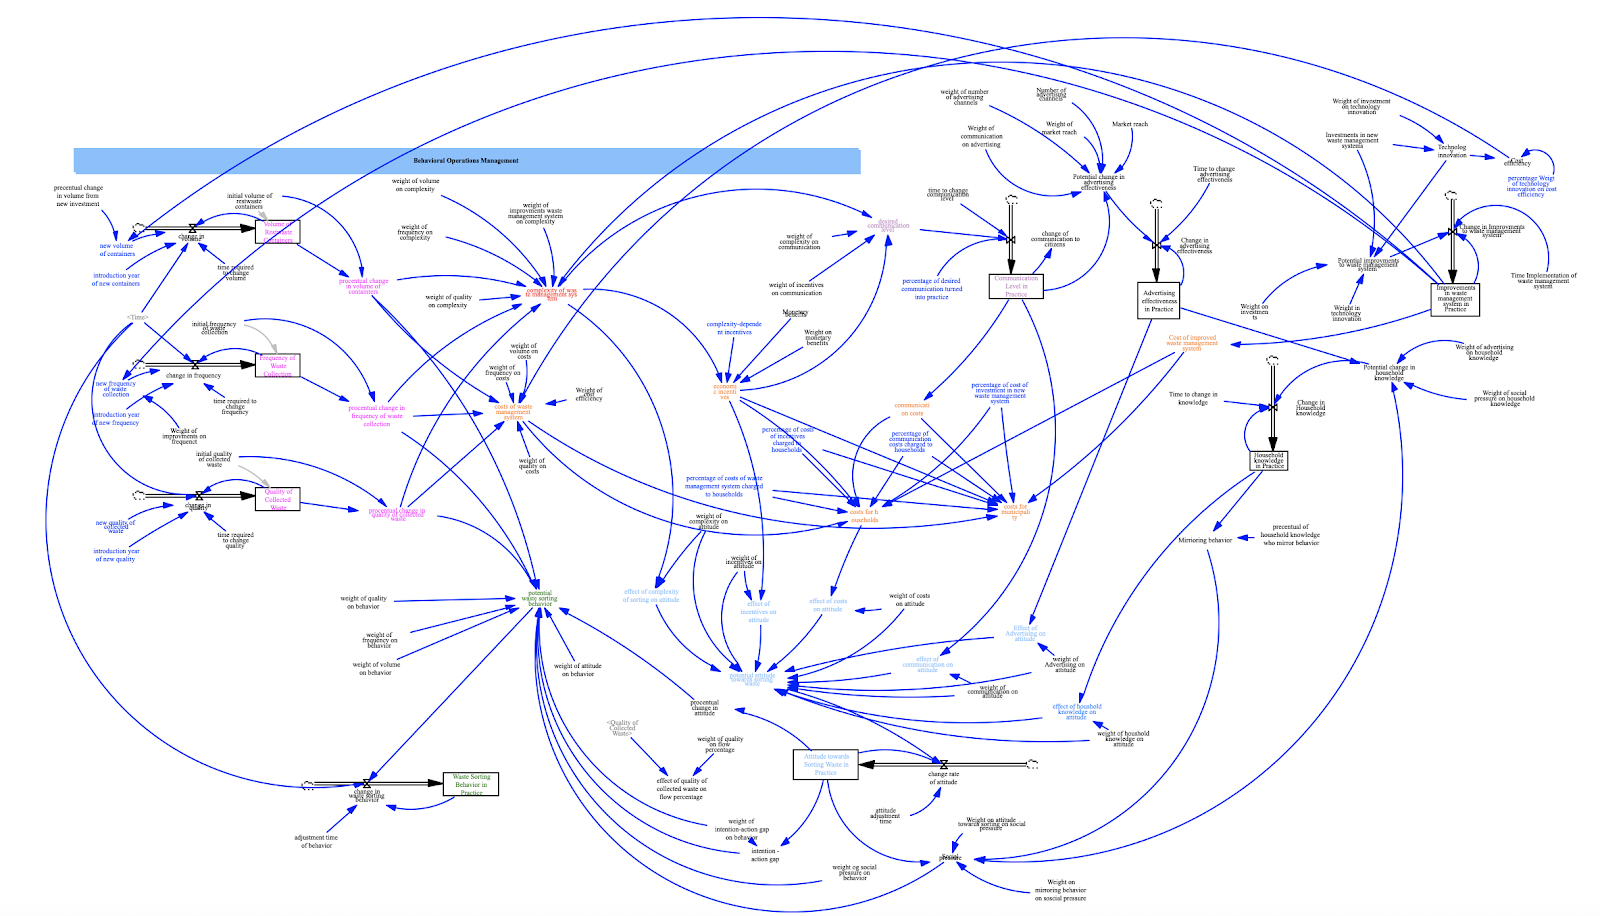
\includegraphics [scale=0.34,angle=90]{figures/overview.png}
\caption{Overview of The Stocks and Flows Model}
\label{fig:overview}
\end{figure}

\indent \newline
Figure 4.4 displays an overview of the complete stocks and flow model, regarding waste sorting behaviour. For further details, please see the attached Vensim file. 


\chapter{Simulation}
The following section describes the simulated base case, with a focus on the key performance indicator (KPI). The KPI represents the material recycling rate, and measures the percentage of household waste, which is recycled. The "base case" simulation does not include any extra efforts from Oslo municipality to influence waste sorting behavior. Note that the simulation only considers food, plastic, rest waste, and paper/cardboard, while glass/metal, textiles and garden waste is excluded. It also only represents the target group, not the whole population in Oslo.  

\indent \newline
Sections later in the chapter presents five recommended initiatives for Oslo municipality to improve the material recycling rate. The effects and outcomes of the practical initiatives will be analyzed and ranked, based on which initiative will have the most effect on waste sorting behavior and the material recycling rate.  

\section{Base Case}

\indent \newline
The "base case" represents a situation without any initiatives from Oslo municipality on waste sorting behavior. The result shows a small increase in the material recycling percentage. As shown in figure 5.1, the material recycling rate increases slightly and reaches 31.69\% by 2030. The graph represents the current state of Oslo's material recycling rate, which will not increase further without extra efforts or initiatives from Oslo municipality. The variable "material recycle percentage" is influenced by how many tons of waste that are collected of each "category", and waste sorting behavior. It is imperative to influence waste sorting behavior in order for the material recycling percentage to increase further. 

\begin{figure}[H]
\centering
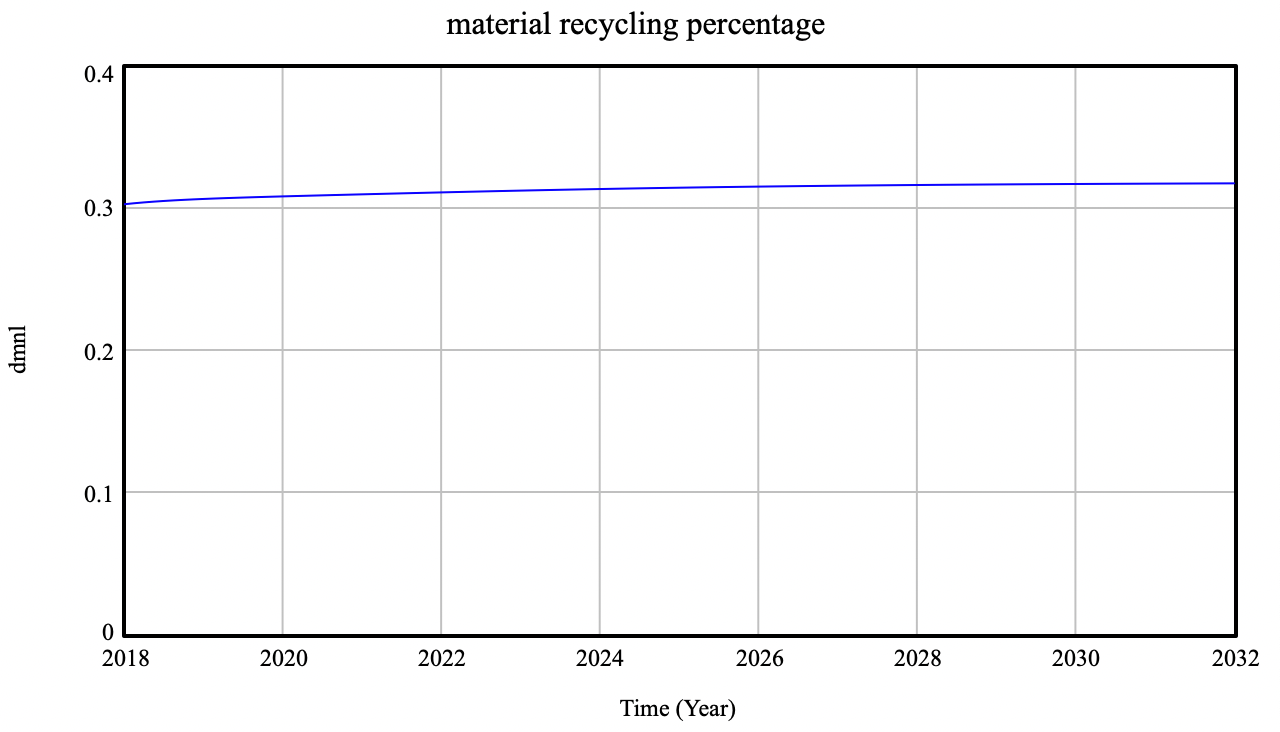
\includegraphics [scale=0.28,angle=360]{figures/basecase.png}
\caption{Base Case}
\label{fig:basecase}
\end{figure}

\indent \newline
The figure above shows that the graph (material recycling percentage) has a steeper increase during the first couple of years, while the graph stagnates when it gets closer to year 2030. This is due to the rate of change in waste sorting behavior. 

\indent \newline
An analyze of figure 5.2 below, demonstrates that the change in waste sorting behavior starts at an elevated level and decreases over time. With comparison to material recycling percentage, the graph stagnates as it moves towards 2030. Waste sorting behavior in practice is determined through the changes in waste sorting behavior. According to the graph, waste sorting behavior in practice has a greater increase during the first couple of years, while it levels out when getting closer to 2030. This is because the target group is adjusting their waste sorting behavior over time. This represents the early adopters of the target group. 

\begin{figure}[H]
\centering
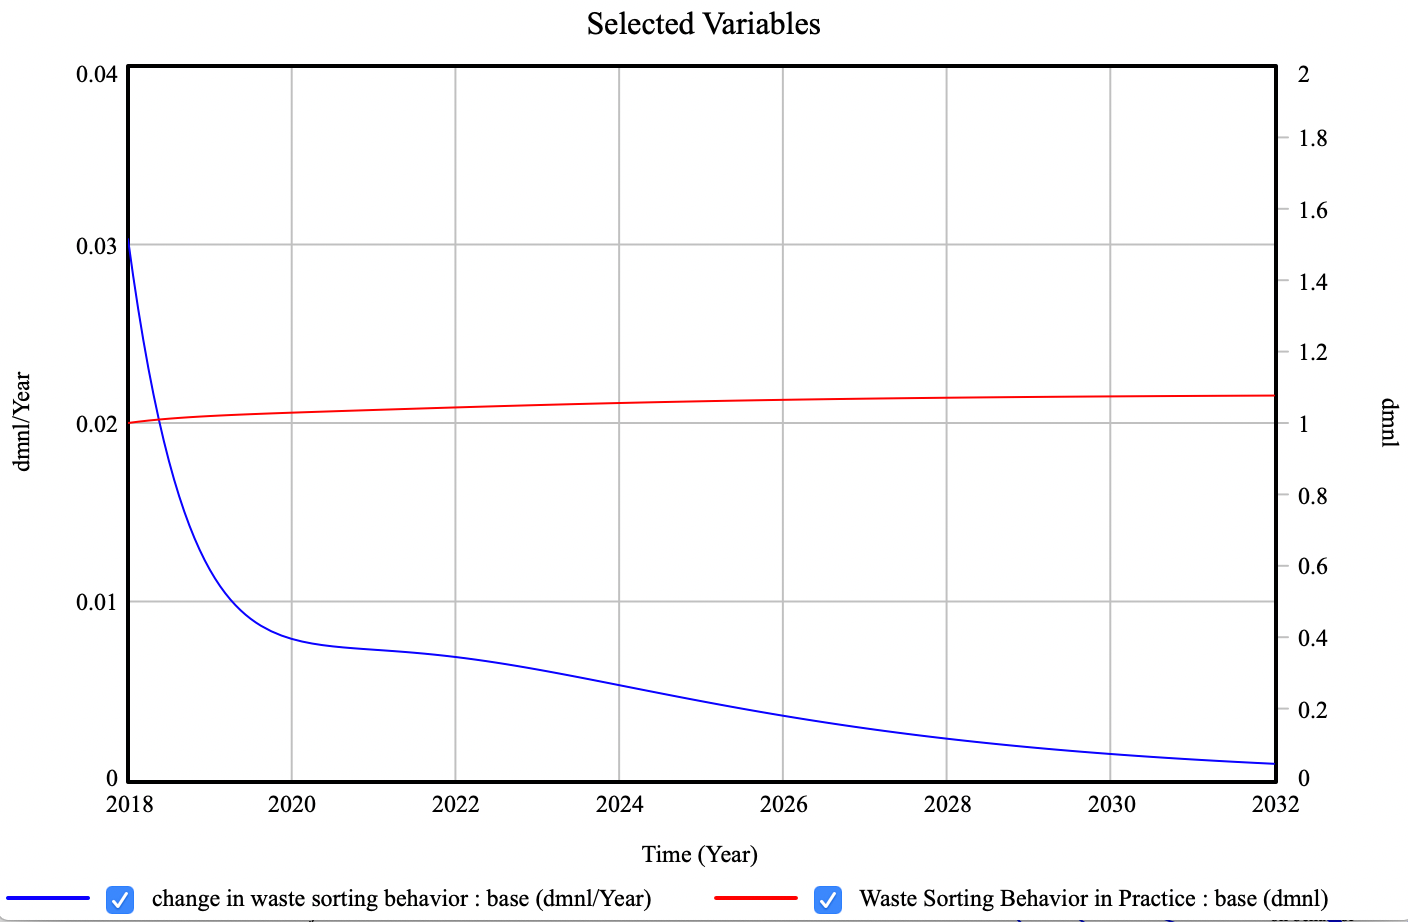
\includegraphics [scale=0.26,angle=360]{figures/basecase2.png}
\caption{Waste Sorting Behavior}
\label{fig:basecase2}
\end{figure}

\indent \newline
The results from the base case simulation indicates that Oslo municipality will not be able to reach the desired recycling rate by 2030. The next part of the chapter describes how the municipality, through additional efforts and initiatives, can improve the recycling percentage in order for them to reach their main goal. 

\section{Initiatives}

\indent \newline
The simulated model is based on five different initiatives Oslo municipality can make use of to improve the recycling percentage. Each of the scenarios is simulated separately to show an isolated effect of the initiatives.

\subsection{Increase Advertising Effectiveness}

\indent \newline
The first initiative consists of increasing advertising effectiveness. It is essential that Oslo municipally increases their marketing spend towards people aged 20-39. Currently, the marketing effect is too low and more effective marketing campaigns in the appropriate channels is needed. Research suggests that the target group needs more information about what the waste goes to after the garbage is thrown \cite[p. 72]{recycling}. The main focus of the marketing will therefore be on explaining the benefits and values of sorting the waste in the right waste container, and the effect of each contribution. 

\indent \newline
In order to reach out to the target group, the municipality should use Snapchat, Facebook, Linkedin, Twitter and Instagram as marketing channels to communicate with the audience. It is also recommended that the communication through these channels consist of the benefits and importance of  recycling waste in the right containers placed in the condominiums. 
The initiative is realistic to implement. Oslo municipality is already doing some advertising at the moment, mostly through television advertisements and Instagram. An assumption is that they already have an advertising department who can start the suggested advertising process, without investing too much in personnel and resources. 

\indent \newline
The target group needs additional information to change their waste sorting behavior. Therefore, a reliable source of information and communication is critical. It is Oslo municipality's responsibility to provide understandable and clear information through these channels. They would answer questions like what and how to sort specific waste. 

\begin{figure}[H]
\centering
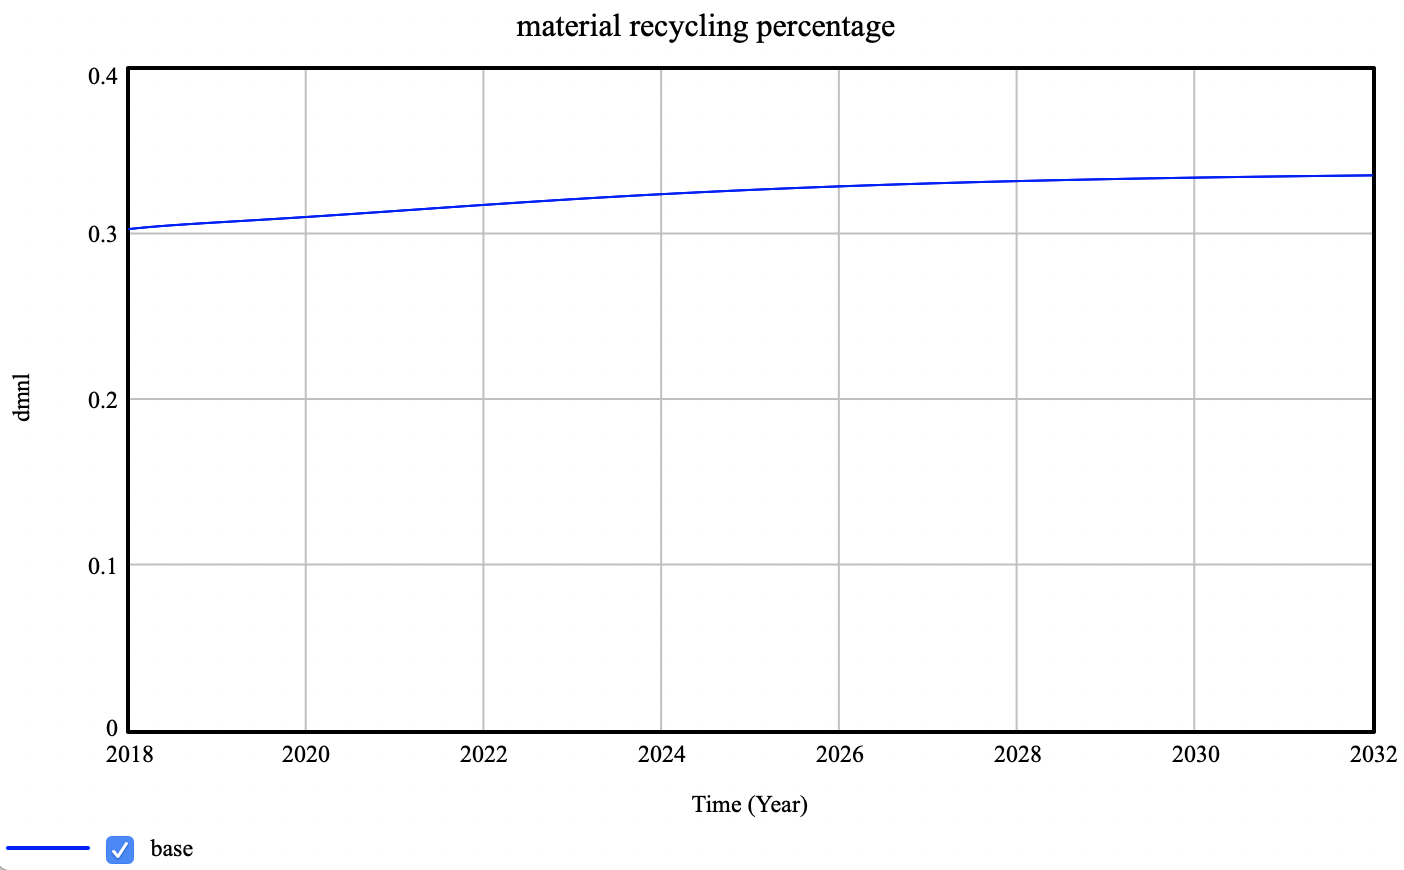
\includegraphics [scale=0.26,angle=360]{figures/advertisingeff.png}
\caption{Increasing Advertising Effectiveness}
\label{fig:advertisingeff}
\end{figure}

\indent \newline
In the figure above, the blue line represents the material recycling percentage and the effect is displayed in the time interval 2018-2030. The graph visualizes an isolated effect of marketing on the recycle percentage, which leads to a final recycling percentage of 33.38\%. Compared to the base case this is an increase of 1.69 percentage points, given that the other variables included in the base case do not affect  the recycling rate. The result shows the effect of marketing in the first 7 years and then the growth rate declines. This reflects that the majority of the market has been reached, which leads to a lower adoption rate. Improvements of the recycling percentage is related to the stock "advertising effectiveness in practice" and the desired goal is to adjust household knowledge and attitude towards waste sorting. As expected, the results indicate a realistic increase in behavior of the target group which affects the recycling percentage. 

\subsection{New Quality of Collected Waste}

\indent \newline
The following initiative represents a situation where there are three waste containers per apartment complex, one for plastic, paper and rest waste. In this scenario, Oslo municipality has to increase the number of waste containers in order to improve the quality of the collected waste. Increasing the quality of collected waste also increases the material recycling percentage, and reduces the amount of residual waste. The main objective in this initiative is providing even better material recycling options. That way, the population can recycle the material in more detail from their homes. This will result in less efforts from Oslo regarding material recycling. 

\begin{figure}[H]
\centering
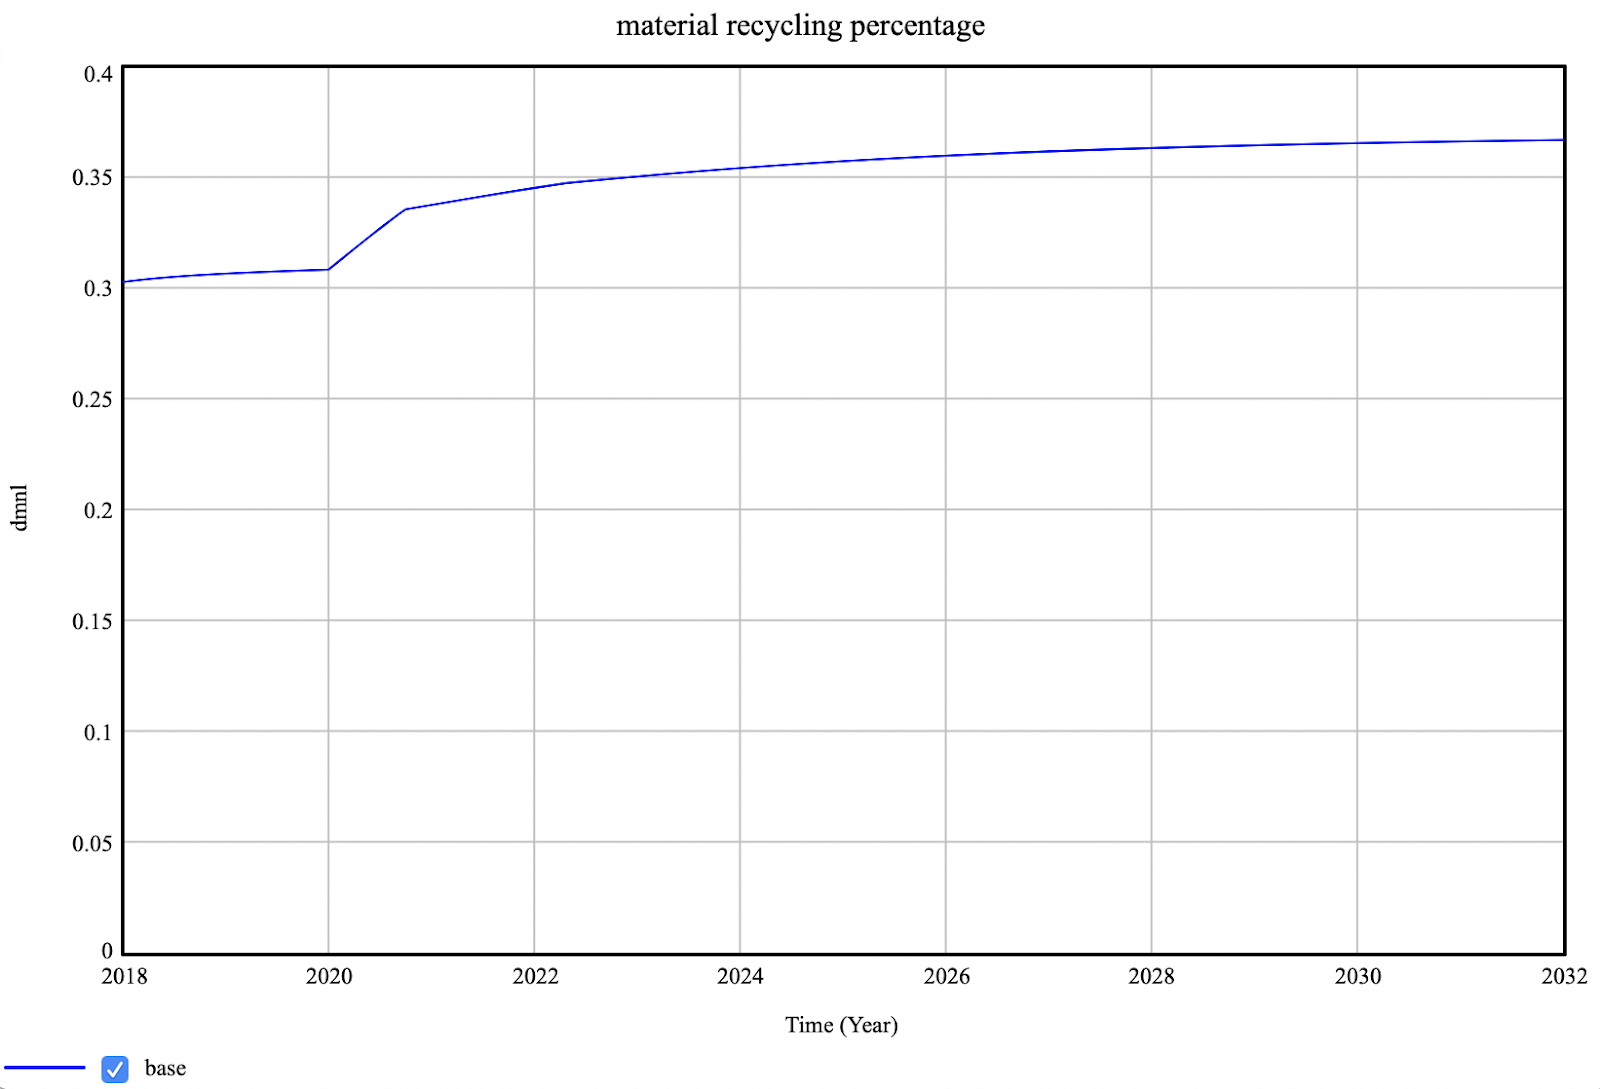
\includegraphics [scale=0.22,angle=360]{figures/newquality.png}
\caption{New Quality of Collected Waste}
\label{fig:newquality}
\end{figure}

\indent \newline
The graph in figure 5.4 represents an isolated effect of an increase of  "quality of collected waste", in other words, the installation of new waste containers. There is a greater increase in the first year, where Oslo municipality introduces new waste containers. After the introduction year, the growth stabilizes due to citizens adapting to the new sorting system. Through implementation of new containers, the recycling percentage increases from 31.69\% in the base case to an improved material recycling percentage of 36.53\%. This results in an increase of 4.84 percentage points and the greatest impact of the initiatives on the model. The implementation of the new containers is represented through the variable "new quality of collected waste", where the initial value is increased from 1 to 2. This means the quality of the sorted waste will increase with 100\%, which might seem like a lot, but it is plausible to assume that more waste containers will have a significant impact on this stock. 

\subsection{Improvements in Waste Management System}

\indent \newline
The third initiative is to implement and utilize smart waste containers for Oslo's apartment buildings. This will ultimately help optimize the frequency of waste collection and the volume of waste containers in the long term. The main concept of the smart containers is that they will automatically compress the waste in the containers. An additional feature is to implement a measuring devices in the waste containers, which will intelligently measure the amount of waste in the containers. The sensors within the containers collect data, which is sent to a server for evaluation and analysis. The results of measurements are displayed in a web platform for the consumers and the waste collection firm to see \cite{smart}

\indent \newline
An additional feature would be to develop an application for smart devices (smart phones, PC, and tablets), where the consumer and collection firm can monitor the current status of the specific waste containers. The consumer will get notified if the container is full, while the waste management company will know when to collect the waste. This data can easily be analyzed, which will help the waste management company to forecast when the container is full, allowing them to plan future routes. The addition of the smart application will increase cost-efficiency and improve the target group's waste sorting behavior. Ultimately, the waste container mechanisms should be driven by solar panel technology, which will help to sustain the system in the long term. 

\begin{figure}[H]
\centering
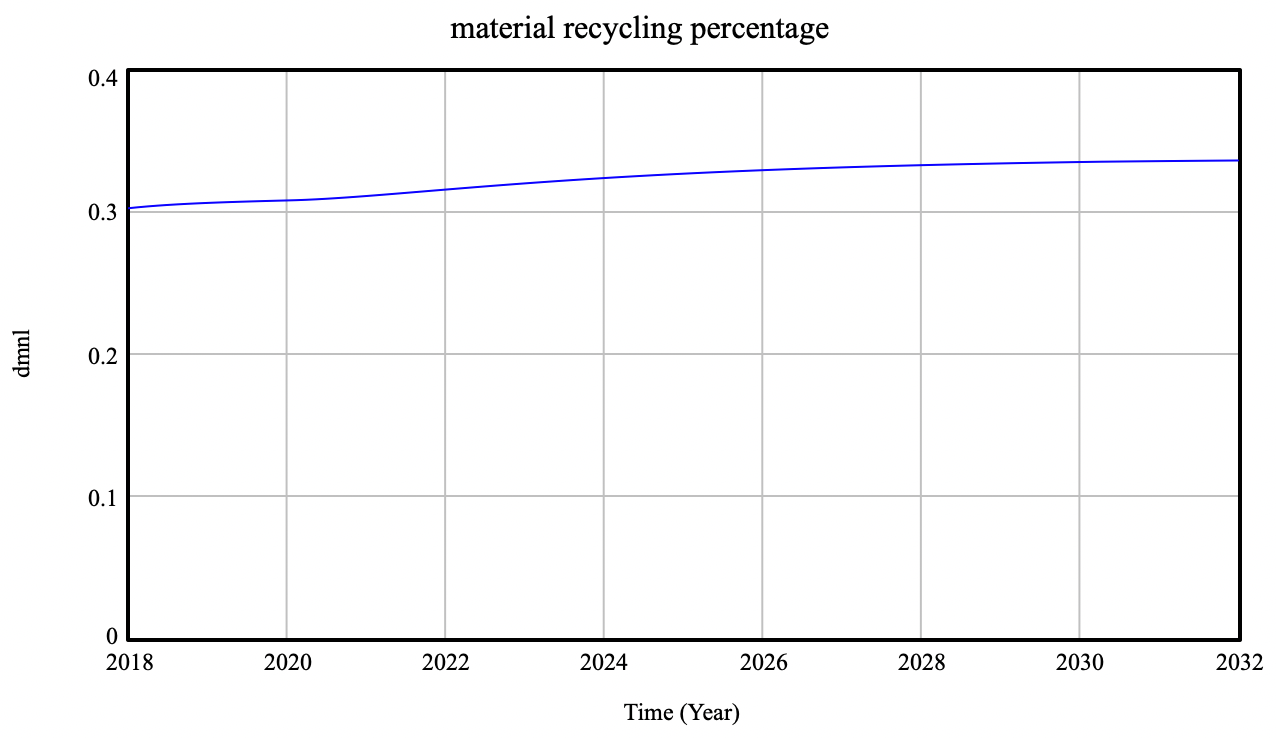
\includegraphics [scale=0.28,angle=360]{figures/improvementsinitiative.png}
\caption{Improvements in Waste Management System}
\label{fig:improvementsinitiative}
\end{figure}

\indent \newline
The simulation results of implementation and utilization of smart containers is displayed in the figure above. Compared to the base case, the effect of smart containers on material recycling percentage is quite positive. An implementation of this initiative leads to an increase in the material recycling rate from the original 31.69\% to 33.86\%. This represents an increase of 2.17 percentage points. The effect of smart containers is implemented in the simulation model through the variable "investments in new waste management system", and increases the value from 1 to 2, which seems to be a realistic value. The implementation of smart containers also positively affects the exogenous variables "new volume of containers" and "new frequency of waste collection". As mentioned earlier, the collection firm can now plan future routes and optimize the frequency of waste collection. They can also simulate patterns for each apartment building and adjust the volume of containers based on the results. The volume is also affected when the containers have the ability to compress the containing waste. 

\indent \newline
The initiative appears to be realistic since the technology already has been developed and being implemented in e.g. Trondheim municipality. There are however implementation costs related to this initiative, but the profit will most likely exceed the costs through optimizing frequency of waste collection and the volume of containers in the long term. 

\subsection{Economic Incentives}

\indent \newline
The fourth initiative is to implement economic incentives to improve the attitude towards waste sorting. According to research, the designated target group would perform better if Oslo municipality provided economic incentives to the residents of apartment complexes \cite[p. 46]{Mikkelborg}. However, it is quite challenging to measure individual waste sorting behavior, as there is no realistic method or system of measuring this. An alternative is to offer a shared economic incentive, based on a given apartment complex. 

\indent \newline
A suggestion is to cut a portion of the shared costs that are related to Oslo municipality's fees and taxes. This will be based on the quality of sorted waste with regards to the apartment building. Furthermore, this would create a culture around waste sorting behavior, and strengthen the community to collaborate to reach the level where economic incentives are generated. This initiative would affect several variables in the long term. Variables such as social pressure, mirroring behavior and intention action gap would either increase or decrease.

\begin{figure}[H]
\centering
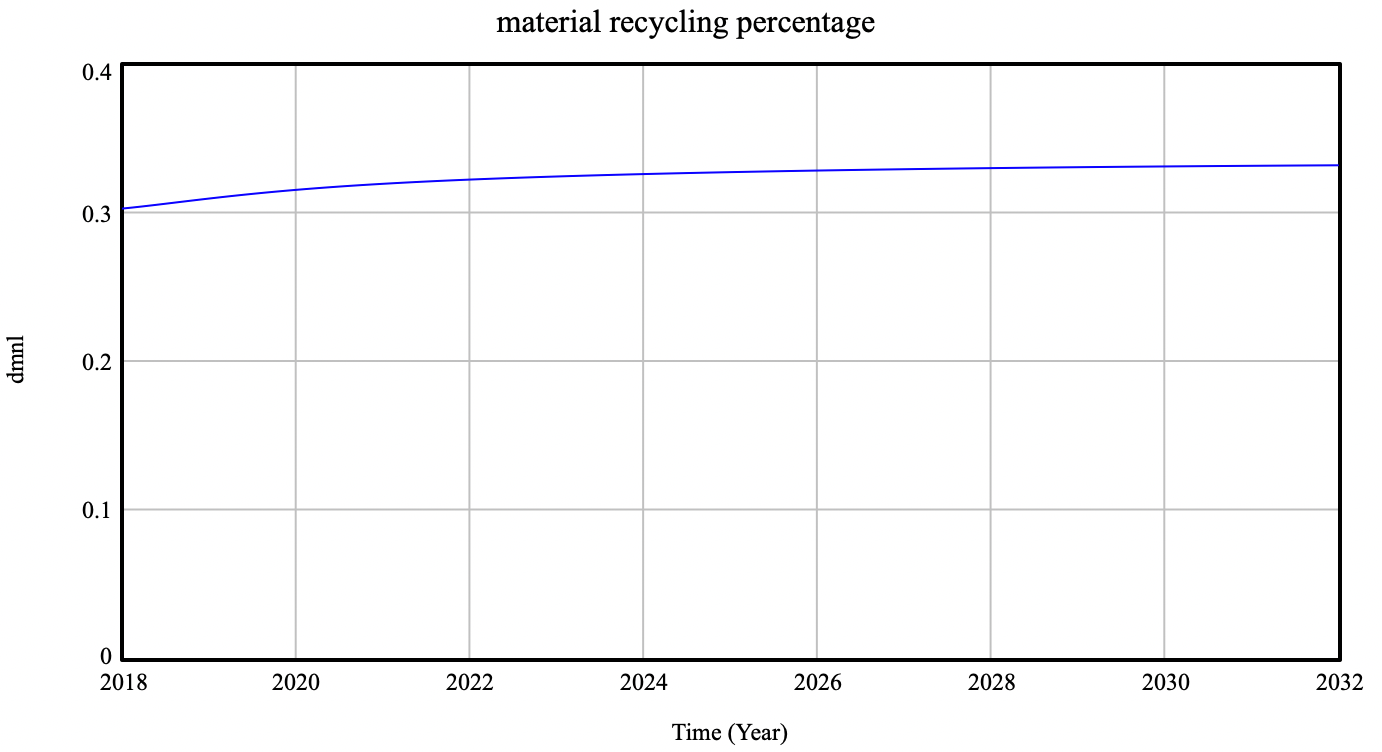
\includegraphics [scale=0.26,angle=360]{figures/incentives.png}
\caption{Economic Incentives}
\label{fig:incentives}
\end{figure}

\indent \newline
In the graph above (figure 5.6), the isolated effect with regards to the implementation of monetary benefits is displayed. Compared to the base case, the material recycle percentage increases from 31.69\% to 33.11\%, which is an increase of 1.42 percentage points. To implement the initiative in the simulation model, the exogenous variable "monetary benefits" is adjusted from 1 to 3. This is a realistic increase, since the target group's motivation will be influenced by monetary benefits. This will also increase the attitude towards waste sorting almost instantly. The implementation of this initiative is both realistic and practical. If Oslo municipality is willing to invest in this initiative, it wouldn't be too challenging to implement. 

\subsection{Increase Frequency of Waste Collection}


\indent \newline
The fifth and final initiative is to increase the frequency of waste collection. Increasing the frequency of waste collection will potentially have a positive influence on waste sorting behavior. There are instances where certain containers get full before the waste collection occurs. This results in garbage bags going in the wrong waste container or being placed on the side/street. Optimizing the waste collection frequency will prevent the waste containers from getting overloaded, and thus improving waste sorting behavior.  

\begin{figure}[H]
\centering
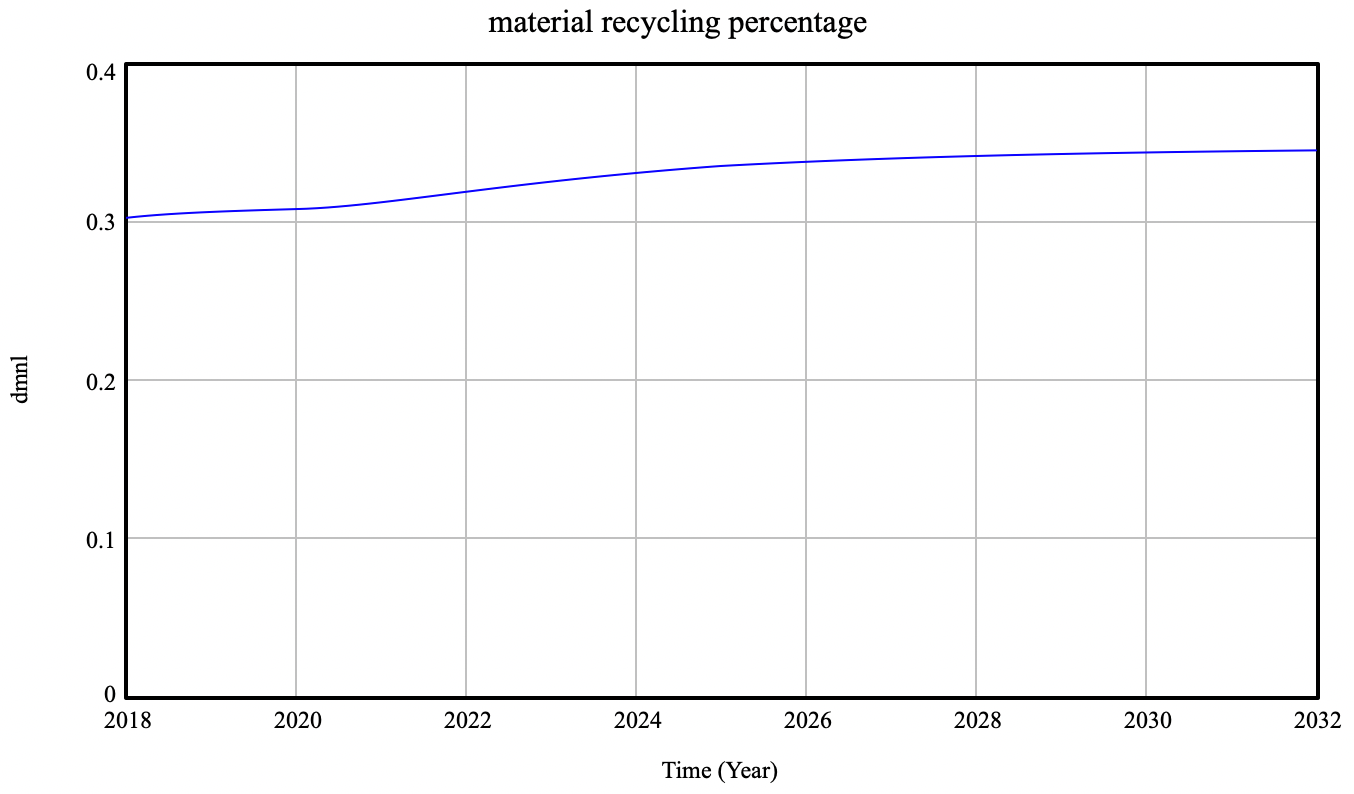
\includegraphics [scale=0.28,angle=360]{figures/frequencyinitiative.png}
\caption{Increasing Frequency of Waste Collection}
\label{fig:frequencyinitiative}
\end{figure}

\indent \newline
The graph in figure 5.7 represents the isolated impact of changing the frequency of waste collection. The material recycling percentage increases from the original 31.69\% to 34.4\%. The total increase in this initiative is 2.71 percentage points. The graph starts out relatively stable and acquires a greater increase after 2020. The reason for this is the variable "introduction year of new frequency". The graph stagnates as it gets closer to 2030 because, by that time, the initiative will have reached its maximum potential. The recommended initiative seems realistic because the implementation of this concept is pretty straight forward, and results in a direct effect on waste sorting behavior. 

\section{Rankings \& Recommendations}

\indent \newline
The figure and table below compares the different initiatives in terms of their effect on the material recycling percentage. The reasoning behind this is to rank the initiatives in order to give the best recommendations to Oslo municipality when it comes to improving the material recycling percentage. 

\begin{figure}[H]
\centering
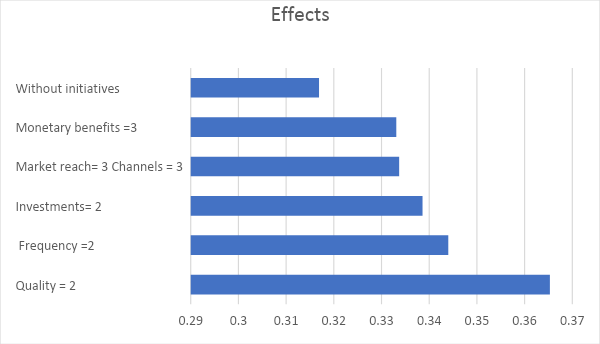
\includegraphics [scale=0.50,angle=360]{figures/rankedinitiatives.png}
\caption{Initiative Scores}
\label{fig:rankedinitiatives}
\end{figure}

\begin{table}[H]
\centering
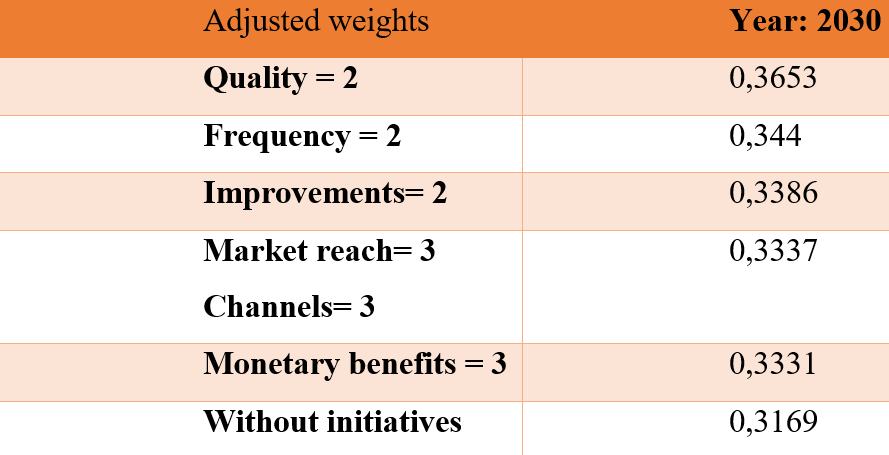
\includegraphics [scale=0.28,angle=360]{tables/rankedinitiatives.png}
\caption{Ranked Initiatives}
\label{tbl:rrankedinitiatives}
\end{table}

\indent \newline
When these five initiatives are separated and simulated individually, there is a similar change in the material recycling percentage. The graphs often have a comparable shape and increases in the interval between 2 and 4 percentage points. Certain initiatives are easier to implement, and therefore takes less time for the effects to kick in. This may, however, result in a reduced impact.

\indent \newline
According to the table above, improving the quality of collected waste is the initiative with the highest impact on the material recycling rate, with a rate of 36.53\%. The second-best initiative is improving the frequency of waste collection, with a rate of 34.4\%. The common denominator between these two initiatives is that they are moderately easy to implement in the real world. It does not require a lot from either Oslo municipality or the consumers. The last of the top 3 initiatives is investing in a new waste management system. This initiative is tougher to implement and execute because it requires more effort and funding from Oslo municipality. The initiative is sustainable in the long term and doesn't require extra efforts from the consumers. It makes life easier for both the collection firm and the target group, with a strong potential for optimizing collection routes. 

\indent \newline
To increase the probability of reaching a 50\% recycling rate by 2030, Oslo municipality should implement these initiatives. Since this paper only focuses on a part of the total population in Oslo, a 50\% recycling rate will be difficult to achieve based on the simulation model. However, these initiatives are still alternatives which will improve the current situation.

\indent \newline
The following part of the paper presents a sensitivity analysis to test the different initiatives in various scenarios.  



\chapter{Sensitivity Analysis}
The sensitivity analysis represents how sensitive the model is to the variation in the value of the variables. The following section explains the effect of the sensitivity analysis on the three initiatives with the best outcomes. The exogenous variables being looked into are "weight of quality on behavior", "weight of attitude on behavior" and "weight of costs on attitude". The simulation focuses on the material recycling percentage in scenarios where the values of the variables are 50\% lower and 50\% higher. 

\indent \newline
When running the simulations, it is clear that the scenarios react in the same pattern. None of the given scenarios regarding the suggested initiatives results in a reduced material recycling percentage.

\begin{table}[H]
\centering
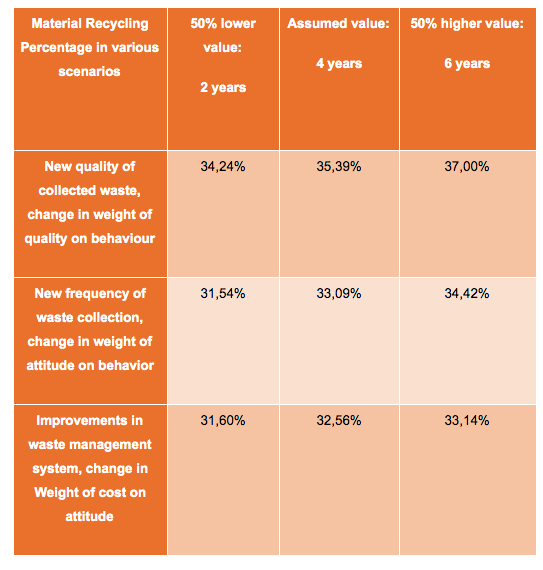
\includegraphics [scale=0.50,angle=360]{tables/scenarios.png}
\caption{Material Recycling Percentage in Different Scenarios}
\label{tbl:scenarios}
\end{table}

\indent \newline
The recommendations from the previous chapter still stands. As measured in the table above, one can clearly state that the new quality of collected waste has the best results in every scenario. For better visualization, please see figures 6.1, 6.2 and 6.3. These figures represent the top three initiatives separately simulated with various values from the exogenous variables at different time slots. 

\indent \newline
Regarding the new quality of collected waste initiative, it has an impact on the material recycle percentage, which makes it interesting to apply a sensitivity analysis. The sensitivity analysis reveals that this initiative is sensitive to a change in the exogenous variable "weight of quality on behavior". Furthermore, the analysis reveals that the model behaves as expected and that it reflects the real world. When increasing the number of waste containers, it should result in a higher material recycling percentage, which is projected in the sensitivity analysis. The initiative "new frequency of waste collection" follows the same pattern as the previous initiative. It is sensitive to an increase in the exogenous variable "weight of attitude on behavior". The third initiative which is reflected through "improvements in waste management system" is also sensitive to the correlated exogenous variable "weight of costs on attitude". It was expected to be sensitive to change, because if Oslo municipality increases the investments, the material recycling percentage will increase as well. 

\indent \newline
The sensitivity analysis shows that adjusting the values related to the exogenous variables and the time-intervals does not change the initial recommendations. The third scenario isn't as sensitive as the previous two initiatives, but still sensitive to some degree. 

\begin{figure}[H]
\centering
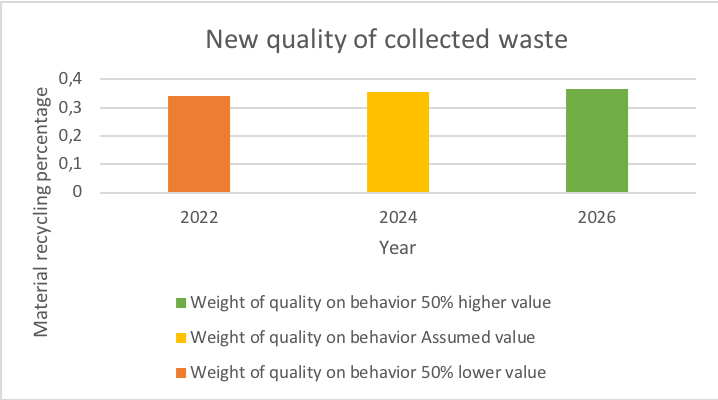
\includegraphics [scale=0.80,angle=360]{figures/sensitivitynew.png}
\caption{Sensitivity Result For New Quality of Collected Waste}
\label{fig:sensitivitynew}
\end{figure}

\begin{figure}[H]
\centering
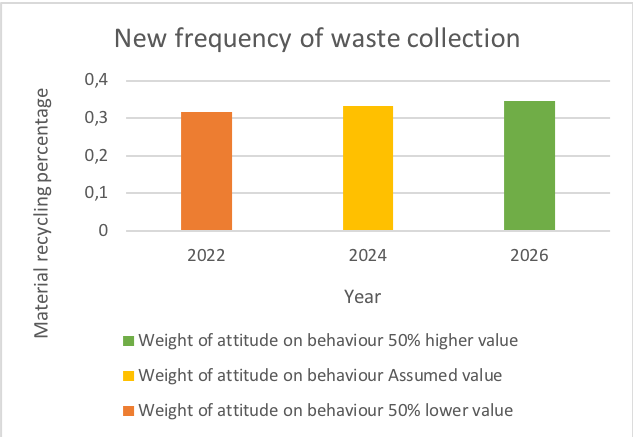
\includegraphics [scale=0.80,angle=360]{figures/sensitivitynewf.png}
\caption{Sensitivity Result For New Frequency of Waste Collection}
\label{fig:sensitivitynewf}
\end{figure}

\begin{figure}[H]
\centering
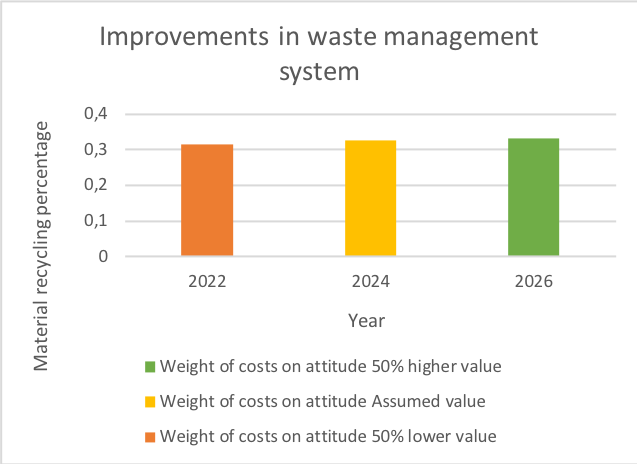
\includegraphics [scale=0.80,angle=360]{figures/sensitivityi.png}
\caption{Sensitivity Result For Improvements in Waste Management System}
\label{fig:sensitivityi}
\end{figure}

% chapter heading as preface and toc
\titleformat{\chapter}[display]
 {\bfseries\Large}
 {}
 {0pt}
 {\color{rockwoolcolor}\titlerule[2.0pt]\vspace{2ex}\filright\color{black}}
 [\color{rockwoolcolor}\vspace{2ex}{\titlerule[2.0pt]}]
 
\renewcommand\bibname{References}
\bibliographystyle{apalike}	% (uses file "plain.bst")
\bibliography{myrefs}		% expects file "mineReferanser.bib"
}

\end{document}
